%!TEX jobname = Master's Degree Dissertation
%!TEX aux_directory = build
%!TEX output_directory = build
%!TEX copy_output_on_build = true
% ---¬
\documentclass[12pt, openright, twoside, a4paper, english, brazil]{USPSC-classe/USPSC}
% ---
% Basic Packages
% ---
\usepackage[T1]{fontenc}
\usepackage[utf8]{inputenc}
\usepackage{lmodern}				
\usepackage{lastpage}
\usepackage{indentfirst}
\usepackage{color}
\usepackage{graphicx}
\usepackage{float} 
\usepackage{tikz}
\usetikzlibrary{positioning}
\usepackage{pdfpages}
\usepackage{makeidx}
\usepackage{hyphenat}
\usepackage[absolute]{textpos}
\usepackage{eso-pic}
\usepackage{makebox}
\usepackage{amsmath}
\usepackage{wrapfig}
\usepackage{setspace}
\usepackage{caption}
\usepackage{subcaption}
\usepackage{physics}
\usepackage{braket}
\usepackage{amssymb}
\usepackage{verbatim}
\usepackage[margin={1.5cm, 1.5cm}]{caption}
% ---

% ---
% Bibliography References
% ---
\usepackage{cite}
\usepackage[num, abnt-emphasize=bf, abnt-thesis-year=both, abnt-repeated-author-omit=no, abnt-last-names=abnt, abnt-etal-cite, abnt-etal-list=3, abnt-etal-text=it, abnt-and-type=e, abnt-doi=doi, abnt-url-package=none, abnt-verbatim-entry=no]{abntex2cite} 
\bibliographystyle{USPSC-classe/abntex2-numeng-USPSC}
% ---

% ---
% Footpage
% ---
%\renewcommand{\thefootnote}{\fnsymbol{footnote}}
\renewcommand{\footnotesize}{\small}
% ---

% ---
% ABNTex2
% ---
\usepackage{multicol}
\usepackage{multirow}
\usepackage{longtable}
\usepackage{threeparttablex}
\usepackage{array}
\usepackage{USPSC-classe/ABNT6023-2018}
% ---

% ---
% Institutional program
% ---
\siglaunidade{IFSC}
\programa{MFAe}
% ---

% ---
% PDF Info
% ---
\definecolor{blue}{RGB}{41,5,195}
\makeatletter
\hypersetup{
	%pagebackref=true,
	pdftitle={\@title}, 
	pdfauthor={\@author},
	pdfsubject={\imprimirpreambulo},
	pdfcreator={LaTeX with abnTeX2},
	pdfkeywords={abnt}{latex}{abntex}{USPSC}{trabalho acadêmico}, 
	colorlinks=true,       		% false: boxed links; true: colored links
	linkcolor=black,          	% color of internal links
	citecolor=black,        		% color of links to bibliography
	filecolor=black,      		% color of file links
	urlcolor=black,
	%Para habilitar as cores dos links, retire a % antes dos comandos abaixo e inclua a % antes das 4 linhas de comando acima 
	%linkcolor=blue,            	% color of internal links
	%citecolor=blue,        		% color of links to bibliography
	%filecolor=magenta,      		% color of file links
	%urlcolor=blue,
	bookmarksdepth=4	
}
\makeatother
% ---

% ---
% Layout
% ---
\setlength{\parindent}{1.3cm}
\setlength{\parskip}{0.2cm}
% ---

% Compile summary and index
% ---
\makeindex
% ---

% Title
% --
\usepackage{titlesec}
% --

% ---
	
% ---
% Document begging
% ---
\begin{document}
	% ---
	% Language
	% ---Since there are only right-handed and left-handed laser beams, $\pi$-transitions do not occur. The $ k_{+} $ and $ k_{-} $ laser beams are exclusively absorbed under some conditionsby $ \sigma_{+} $	 and $ \sigma_{-} $ transitions respectively.
	\selectlanguage{english}
	\vspace{5pt}
	% ---

	% ---
	% Formatting
% 	% ---fig:1D-MOT
	\frenchspacing
	\renewcommand{\ABNTEXchapterfontsize}{\fontsize{12}{12}\bfseries}
	\renewcommand{\ABNTEXsectionfontsize}{\fontsize{12}{12}\bfseries}
	\renewcommand{\ABNTEXsubsectionfontsize}{\fontsize{12}{12}\normalfont}
	\renewcommand{\ABNTEXsubsubsectionfontsize}{\fontsize{12}{12}\normalfont}
	\renewcommand{\ABNTEXsubsubsubsectionfontsize}{\fontsize{12}{12}\normalfont}
	% ---

	% ----------------------------------------------------------
	% PRE-TEXTUAL ELEMENTS
	% ----------------------------------------------------------

	\imprimircapa
	\imprimirfolhaderosto*

	%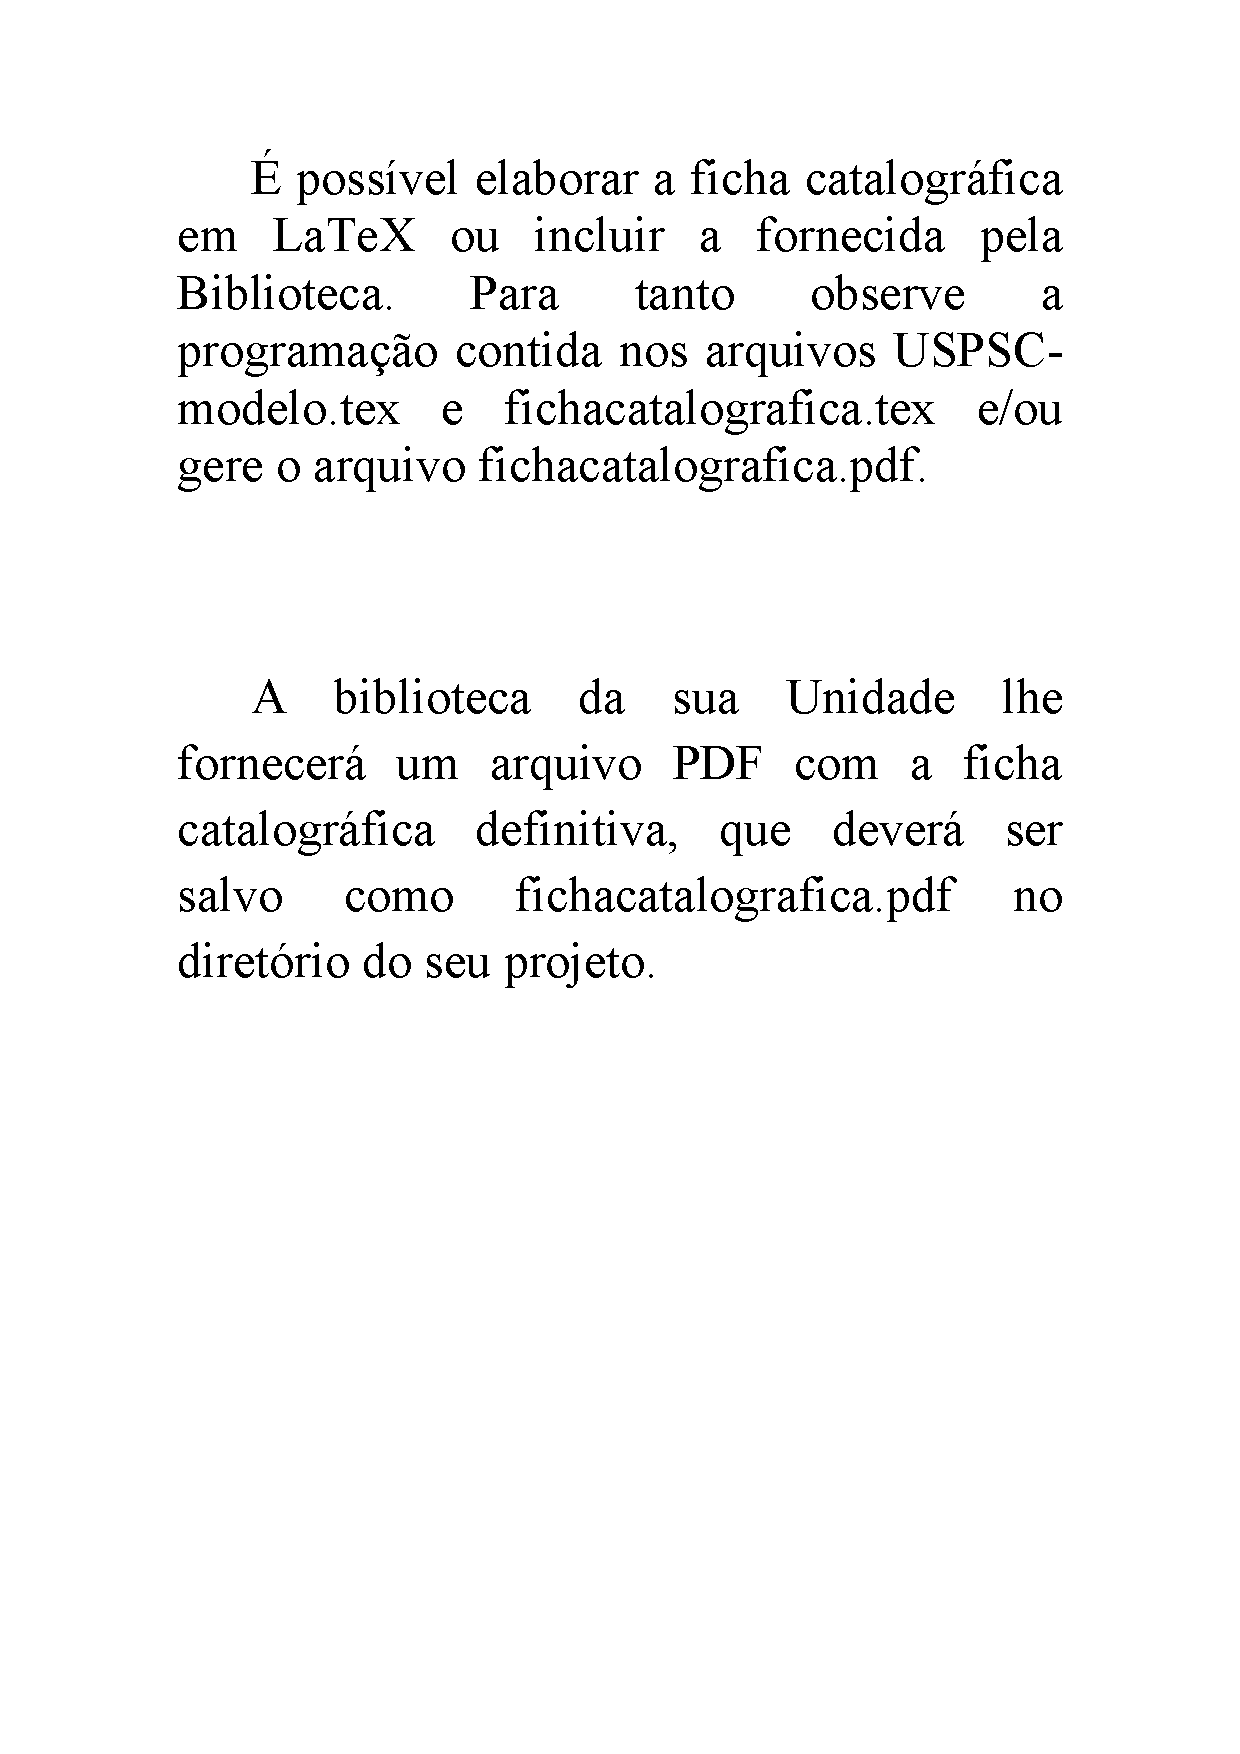
\includepdf{USPSC-TA-PreTextual/USPSC-fichacatalografica.pdf}
	%%% USPSC-Errata.tex
\begin{errata}
	%\OnehalfSpacing 			
	A errata é um elemento opcional, que consiste de uma lista de erros da obra, precedidos pelas folhas e linhas onde eles ocorrem e seguidos pelas correções correspondentes. Deve ser inserida logo após a folha de rosto e conter a referência do trabalho para facilitar sua identificação, conforme a ABNT NBR 14724 \cite{nbr14724}.
	
	Modelo de Errata:
		
	\begin{flushleft} 
			\setlength{\absparsep}{0pt} % ajusta o espaçamento da referência	
			\SingleSpacing 
			\imprimirautorabr~ ~\textbf{\imprimirtituloresumo}.	\imprimirdata. \pageref{LastPage}p. 
			%Substitua p. por f. quando utilizar oneside em \documentclass
			%\pageref{LastPage}f.
			\imprimirtipotrabalho~-~\imprimirinstituicao, \imprimirlocal, \imprimirdata. 
 	\end{flushleft}
\vspace{\onelineskip}
\OnehalfSpacing 
\center
\textbf{ERRATA}
\vspace{\onelineskip}
\OnehalfSpacing 
\begin{table}[htb]
	\center
	\footnotesize
	\begin{tabular}{p{2cm} p{2cm} p{4cm} p{4cm} }
		\hline
		\textbf{Folha} & \textbf{Linha}  & \textbf{Onde se lê}  & \textbf{Leia-se}  \\
			\hline
			1 & 10 & auto-conclavo & autoconclavo\\
		\hline
	\end{tabular}
\end{table}
\end{errata}
% ---
	%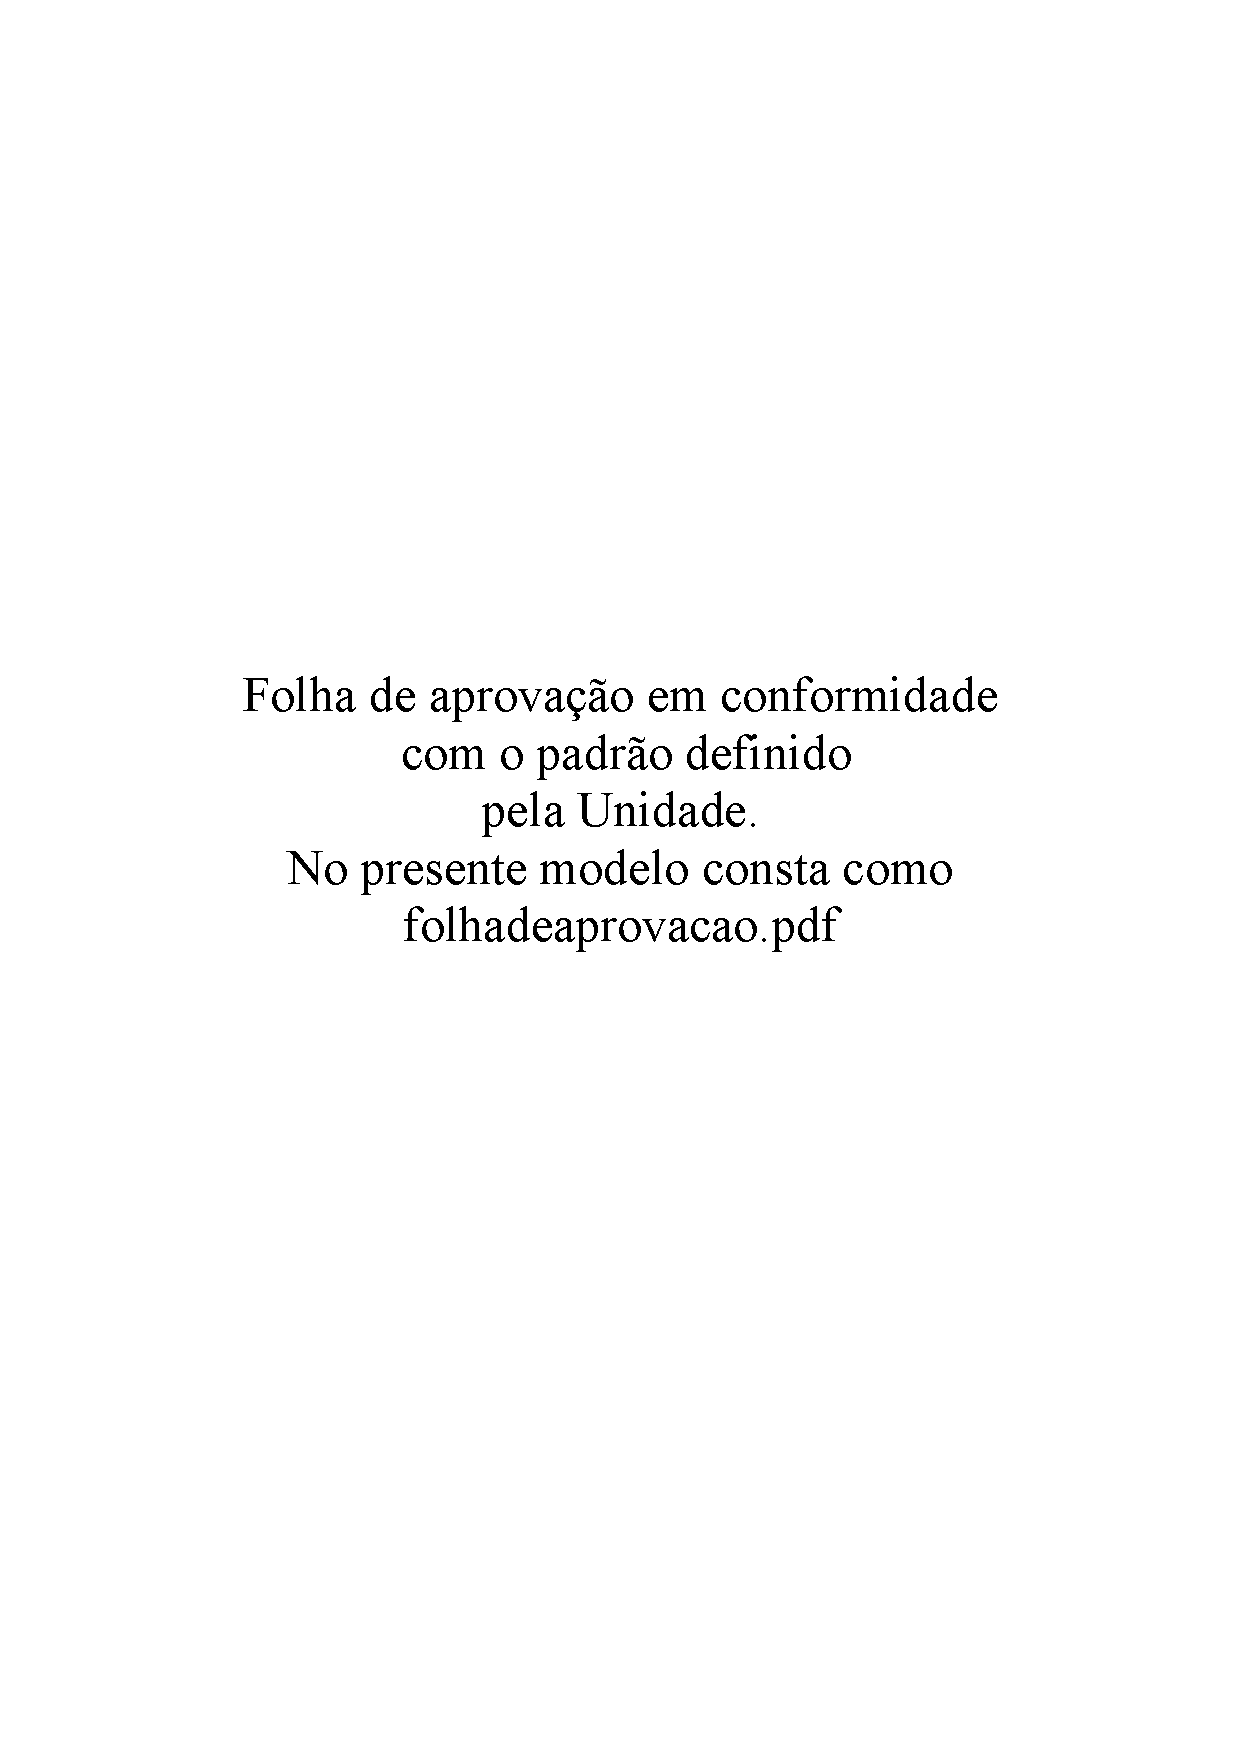
\includepdf{USPSC-TA-PreTextual/USPSC-folhadeaprovacao.pdf}
	%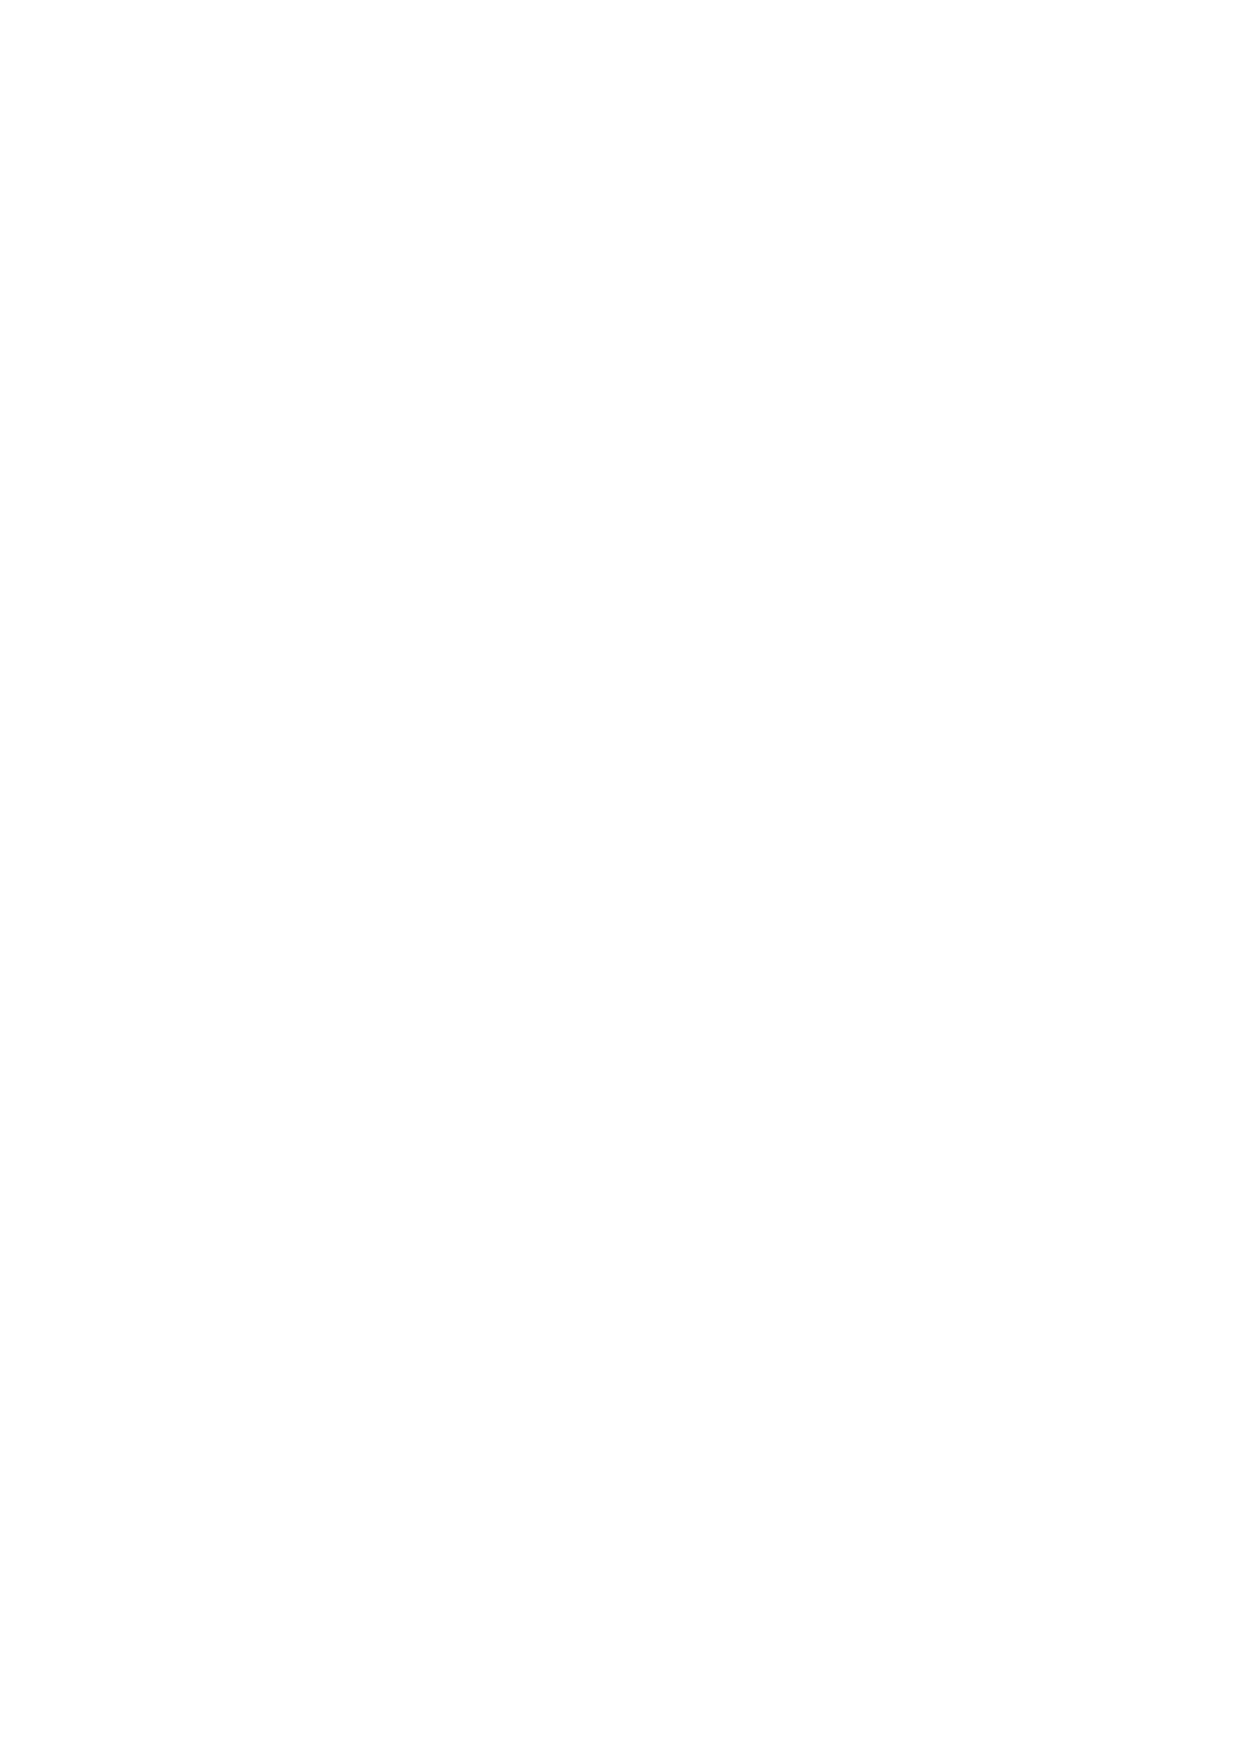
\includepdf{USPSC-TA-PreTextual/USPSC-PaginaEmBranco.pdf}

	% ---
	% Dedication
	% ---
	%%% USPSC-Dedicatoria.tex
\begin{dedicatoria}
   \vspace*{\fill}
   \centering
   \noindent
   \textit{For my family and friends who support me during all my academic life.} \vspace*{\fill}
\end{dedicatoria}
% ---
	% ---

	% ---
	% Thanks
	% ---
	%%% USPSC-Agradecimentos.tex
\begin{agradecimentos}
	Primeira frase do agradecimento ....
	
	Segunda frase ....
	
	Outras frases ....
	
	Última frase ....
	
\end{agradecimentos}
% ---
	% ---

	% ---
	% Epigraph
	% ---
	%%% USPSC-Epigrafe.tex
\begin{epigrafe}
    \vspace*{\fill}
	\begin{flushright}
		\textit{``O estudo, a busca da verdade e da beleza são domínios \\
		em que nos é consentido sermos crianças por toda a vida.''\\
		Albert Einstein}
	\end{flushright}
\end{epigrafe}
% ---
	% ---

	% English Abstract
	% ---
	%%% USPSC-Abstract.tex
%\autor{Silva, M. J.}
\begin{resumo}[Abstract]
 \begin{otherlanguage*}{english}
	\begin{flushleft} 
		\setlength{\absparsep}{0pt} % ajusta o espaçamento dos parágrafos do resumo		
 		\SingleSpacing  		\imprimirautorabr~~\textbf{\imprimirtitleabstract}.	\imprimirdata.  \pageref{LastPage}p. 
		%Substitua p. por f. quando utilizar oneside em \documentclass
		%\pageref{LastPage}f.
		\imprimirtipotrabalhoabs~-~\imprimirinstituicao, \imprimirlocal, 	\imprimirdata. 
 	\end{flushleft}
	\OnehalfSpacing 
   This is the english abstract.

   \vspace{\onelineskip}
 
   \noindent 
   \textbf{Keywords}: LaTeX. USPSC class. Thesis. Dissertation. Conclusion course paper. 
 \end{otherlanguage*}
\end{resumo}

	% --- 

	% ---
	% Portuguese Abstract
	% ---
	%%% USPSC-Resumo.tex
\setlength{\absparsep}{18pt} % ajusta o espaçamento dos parágrafos do resumo		
\begin{resumo}
	\begin{flushleft} 
			\setlength{\absparsep}{0pt} % ajusta o espaçamento da referência	
			\SingleSpacing 
			\imprimirautorabr~~\textbf{\imprimirtituloresumo}.	\imprimirdata. \pageref{LastPage}p. 
			%Substitua p. por f. quando utilizar oneside em \documentclass
			%\pageref{LastPage}f.
			\imprimirtipotrabalho~-~\imprimirinstituicao, \imprimirlocal, \imprimirdata. 
 	\end{flushleft}
\OnehalfSpacing 			
 O resumo deve ressaltar o  objetivo, o método, os resultados e as conclusões do documento. A ordem e a extensão  destes itens dependem do tipo de resumo (informativo ou indicativo) e do  tratamento que cada item recebe no documento original. O resumo deve ser
 precedido da referência do documento, com exceção do resumo inserido no
 próprio documento. (\ldots)  Salientamos que algumas Unidades exigem o titulo dos trabalhos acadêmicos em inglês, tornando necessário a inclusão das referências nos resumos e abstracts, o que foi adotado no \textbf{Modelo para TCC em \LaTeX\ utilizando a classe USPSC} e no \textbf{Modelo para teses e dissertações em \LaTeX\ utilizando a classe USPSC}. As palavras-chave devem figurar logo abaixo do  resumo, antecedidas da expressão Palavras-chave:, separadas entre si por  ponto e finalizadas também por ponto \cite{nbr6028}.
 

 \textbf{Palavras-chave}: LaTeX. Classe USPSC. Tese. Dissertação. Trabalho de conclusão de curso (TCC). 
\end{resumo}
	% ---

	% ---
	% Pictures list
	% ---
	\pdfbookmark[0]{\listfigurename}{lof}
	\listoffigures*
	\cleardoublepage
	% ---

	% ---
	% Tables list
	% ---
	%\pdfbookmark[0]{\listtablename}{lot}
	%\listoftables*
	%\cleardoublepage
	% ---

	% ---
	% Boards list
	% ---
	%\pdfbookmark[0]{\listofquadroname}{loq}
	%\listofquadro*
	%\cleardoublepage
	% ---

	% ---
	% Abbreviation
	% ---
	%% USPSC-AbreviaturasSiglas.tex
\begin{siglas}
    \item[ABNT] Associação Brasileira de Normas Técnicas
    \item[abnTeX] ABsurdas Normas para TeX
	\item[IBGE] Instituto Brasileiro de Geografia e Estatística
	\item[LaTeX] Lamport TeX
	\item[USP] Universidade de São Paulo
	\item[USPSC] Campus USP de São Carlos
\end{siglas}

	% ---

	% ---
	% Symbols
	% ---
	%% USPSC-Simbolos.tex
\begin{simbolos}
  \item[$ \Gamma $] Letra grega Gama
  \item[$ \Lambda $] Lambda
  \item[$ \zeta $] Letra grega minúscula zeta
  \item[$ \in $] Pertence
\end{simbolos}
	% ---

	% ---
	% Summary
	% ---
	\pdfbookmark[0]{\contentsname}{toc}
	\tableofcontents*
	\cleardoublepage
	% ---

	% ----------------------------------------------------------
	% Textual Elements
	% ----------------------------------------------------------
	\textual

	% ---
	% Introduction
	% ---
	%
%
% Introduction Section
%-----------------------------------
\chapter{Introduction}
\label{ch:introduction}
%-----------------------------------

The deep understanding of light-matter interaction brought several scientific possibilities such as improvements in the atom interferometry \cite{peters2001high}, accurate spectroscopic methods \cite{mukamel2020roadmap}, and control of ultracold atoms. 
The Nobel Prize in Physics of 1997 was awarded jointly to Steven Chu \cite{chu1998nobel}, Claude Cohen-Tannoudji \cite{cohen1998nobel}, and William D. Phillips \cite{phillips1998nobel} for developing methods to cool and trap atoms with laser light, also known as laser cooling \cite{metcalf2007laser}. This achievement has enabled modern technologies, including accurate atomic clocks \cite{ludlow2015optical}, qubits for quantum computing \cite{schneider2012quantum}, and quantum sensors \cite{zhang2016precision}. Laser cooling also allowed the experimental confirmation of the Bose-Einstein condensation (BEC), motivating the Nobel Prize of Physics in 2001 \cite{cornell2002nobel, ketterle2002nobel}.

The workhorse of laser cooling is the magneto-optical trap (MOT) \cite{krzysztof2010magneto}, a technique to trap and cool a dilute atomic gas until temperatures in a range of $\mu K$. A standard MOT consists of three pairs of counter-propagating laser beams mutually orthogonal and a magnetic quadrupole field. Briefly, the atoms scatter photons from the laser light through atomic transitions, which cause momentum exchanges. The average momentum exchange yields a trapping and drag force on the atoms (MOT force), whereas its fluctuations determine temperature. The frequency of these random scatterings increases with the atomic linewidth and defines the magnitude of both MOT force and fluctuations. Hence, MOTs operating with narrow transitions reach lower temperatures at the cost of trapping efficiency. When the linewidth is comparable to the photonic recoil, we have the narrow line magneto-optical trap (nMOT) \cite{frisch2012narrow, maier2014narrow, miyazawa2021narrow}.

\textcolor{red}{In practice, the study of the MOT force without the two-level system approximation often involves numerical simulations or more advanced theoretical techniques such as density matrix equations or Monte Carlo methods. These approaches can provide insights into the MOT dynamics by taking into account the complete energy level structure and the complex interactions involved.}

The current MOT theories based upon Doppler cooling are rather limited to predict quantities such as temperature \cite{lett1988observation} and atomic cloud size \cite{gattobigio2010scaling}. In many experiments, there is either the absence of theoretical predictions or the necessity of adjustable scaling factors \cite{loo2003investigations}. Furthermore, most of these theories are restricted to an unfeasible one-dimensional MOT \cite{metcalf2007laser, balykin2000electromagnetic}. The difficulty arises from the three-dimensional laser beams arrangement in the presence of a magnetic quadrupole field. There are few papers devoted to develop a 3D MOT model \cite{prudnikov2015three}, all of them with strong limitations. The case of nMOTs is even more delicate since gravity can be comparable with the optical forces and then must be included. Therefore, it is evident that a computational approach to predict MOT features is appropriate and often required \cite{chaudhuri2006realization, atutov2001sodium,hanley2018quantitative}.

In this thesis, we focus perform a deep analysis of the atom dynamics in nMOTs through a stochastic simulation proposal. Our model relies on sampling ensembles of random atomic trajectories as a discrete stochastic process, more precisely as a Markov chain. To validate the model, we simulate standard six-beam nMOTs of dysprosium and strontium, obtaining results in agreement with experimental measurements. Then we analyze the nuances of the stochastic dynamics in nMOTs based upon simulated data.

%-----------------------------------
\section{The thesis}
\label{sec:introduction-thesis}
%-----------------------------------

In the framework of this thesis, we execute a deep study of atom-light interactions and stochastic processes aiming to understand the atom dynamics from both optical forces and photon scattering (Markovian process) perspectives. The radiation pressure force is the base of the Doppler cooling theory, whereas the stochastic dynamics theory is essential to computationally approach the atoms dynamics and then infer experimental quantities.

Firstly, we investigate the basic concepts of atom-light interaction through the Einstein rate equations. Although this approach is proper to attend an elementary understanding, it does not contemplate coherent effects such as Rabi oscillations and the nature of line broadening mechanisms. To take these phenomena into account, we introduce the density operator formalism, treating the atom-light interaction semiclassically. Afterwards, we introduce both radiation pressure force and gradient dipole force, also known as optical forces. Finally, we verify the conditions to occur a transition between electronic states.

\textcolor{red}{Study of magneto-optical traps and the limit of narrow-line}

\textcolor{red}{Study of stochastic dynamics in nMOTs}

\textcolor{red}{Comments about results}

	% ---

	% ---
	% Light-Matter Interaction
	% ---
	%
%--- 
%-----------------------------------
\chapter{Atom-light interaction}
\label{ch:atom-light-interaction}
%-----------------------------------
%--- 
%

In this chapter, we review several aspects of atom-light interaction \cite{weiner2003light} to properly approach the stochastic atomic dynamics in magneto-optical traps. First of all, we shall explore the basic concepts through \textbf{the phenomenological Einstein rate equations} \cite{foot2005atomic}, a "semi-quantum" model where atoms absorb and emit light at a defined rate. Afterwards, we invoke the quantum mechanics apparatus through the \textbf{density operator} and the \textbf{master equation} \cite{steck2007quantum} to analyze coherence effects and line broadening mechanisms. We minutely approach the case of a two-level atom interacting with a monochromatic radiation through the semiclassical approach. Finally, we brief discuss conditions in which electric dipole transitions are allowed.


% Rate Equations Model
%-----------------------------------
%
%-----------------------------------
\section{Rate equations model}
\label{sec:rate-equations-model}
%-----------------------------------
%

A simple approach to introduce the essential aspects of atom-light interaction was proposed by Einstein in 1917. Although this theory does not take coherent effects into account, it is justified within the quantum mechanics framework in appropriate limits. Einstein assumed discrete energy levels for both atom and light. In this context, the electromagnetic radiation is composed of packets of energy $ \hbar \omega $ and momentum $ \hbar \omega / c $ known as photons, where $ \omega $ is the angular frequency, $ \hbar = h / 2\pi$ is the reduced Planck constant, and $ c $ is the speed of light. Einstein also postulated phenomenological rate equations to describe two-level atomic transitions due to the absorption and emission of photons. Let us consider a two-level transition where the energy difference between the upper and lower level is $ \hbar \omega_0 $, and an electromagnetic radiation with spectral energy density $ u(\omega) $. In Figure \ref{fig:optical-transitions}, we illustrated the three possible transitions involving absorption and emission of photons.

Let us consider a dilute atomic gas with number density $ n_1(t) $ of atoms in the lower level and number density $ n_2(t) $ of atoms in the upper level after a period of time $ t $. The Einstein rate equations express the time evolution of $ n_1 $ and $ n_2 $ so that
\begin{equation}
	\frac{d n_1}{dt} = - \frac{d n_2}{dt} = - B_{12} u(\omega_0) n_1 + B_{21} u(\omega_0) n_2 + A n_2,
	\label{eq:Einstein-rate-equations}
\end{equation}
where $ B_{12} u(\omega_0) $, $ B_{21} u(\omega_0) $, and $ A $ are phenomenological rates associated with the stimulated absorption, stimulated emission and spontaneous emission respectively. The rates associated with stimulated processes are proportional to the spectral density energy and therefore theses processes only happen in the presence of a light field. 

\begin{figure}[H]
	\caption{Optical two-level transitions}
	\begin{subfigure}[t]{0.32\textwidth}
		\centering
		\subcaption{\textbf{Stimulated absorption}}
		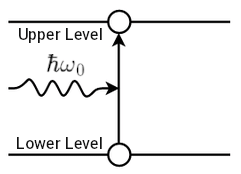
\includegraphics[width=0.8\textwidth]{USPSC-img/stimulated_absorption.png}
		\vspace{5pt}
		\legend{An atom in the lower level goes into the upper level absorbing a photon with energy $ \hbar \omega_0 $ from a light field with $ u(\omega_0) > 0 $.}
		\label{img:stimulated-absorption}
	\end{subfigure}
	\hfill
	\begin{subfigure}[t]{0.32\textwidth}
		\centering
		\subcaption{\textbf{Stimulated emission}}
		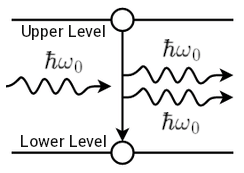
\includegraphics[width=0.8\textwidth]{USPSC-img/stimulated_emission.png}
		\vspace{5pt}
		\legend{An atom in the upper level decays into the lower level in the presence of a light field with $ u(\omega_0) > 0 $, emitting a photon with energy $\hbar \omega_0 $ similar to the photons in the light field.}
		\label{img:stimulated-emission}
	\end{subfigure}
	\hfill
	\begin{subfigure}[t]{0.32\textwidth}
		\centering
		\subcaption{\textbf{Spontaneous emission}}
		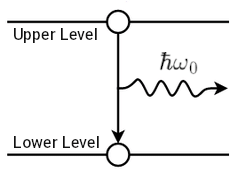
\includegraphics[width=0.8\textwidth]{USPSC-img/spontaneous_emission.png}
		\vspace{5pt}
		\legend{An atom in the upper level emits an isotropic photon with energy $ \hbar \omega_0 $ spontaneously, decaying into the lower level.}
		\label{img:spontaneous-emission}
	\end{subfigure}

	\legend{Source: Author}
	\vspace{-20pt}
	\label{fig:optical-transitions}
\end{figure}

%
%-----------------------------------
\subsection{Relation between the Einstein coefficients}
%-----------------------------------
%

A dilute atomic gas at temperature $ T $ in thermal equilibrium establishes a steady state in which $ n_1 $ and $ n_2 $ are constants of time ($ d_{t} n_1 = - d_{t} n_2 = 0 $). In this condition, from equation (\ref{eq:Einstein-rate-equations}), the spectral energy density is
\begin{equation}
	u({\omega_0}) = \frac{A}{(n_1 / n_2) B_{12} - B_{21}}.
	\label{eq:spectral-energy-thermal-equilibrium}
\end{equation}
Considering a fixed number of atoms $ n = n_1 + n_2 $, the system are represented by the canonical ensemble and then the ratio $ n_1 / n_2 $ is associated with the Boltzmann distribution so that
\begin{equation}
	\frac{n_1}{n_2} = \frac{g_1}{g_2} \exp\left\{-\frac{\hbar \omega_0}{k_B T}\right\},
	\label{eq:Boltzmann-distribution}
\end{equation}
where $ g_1 $ and $ g_2 $ are the degeneracies of the lower and upper level, respectively, and $ k_B $ is the Boltzmann constant. Einstein evaluated atoms in a region of black body radiation,  in which the spectral energy density of the light is consistent with the Planck distribution law given by
\begin{equation}
	u(\omega_0) = \frac{\hbar \omega_0^3}{\pi^2 c^3} \frac{1}{e^{\hbar \omega_0 / k_B T} - 1}.
	\label{eq:Planck-distribution}
\end{equation}
Comparing (\ref{eq:spectral-energy-thermal-equilibrium}), (\ref{eq:Boltzmann-distribution}), and (\ref{eq:Planck-distribution}), we obtain
\begin{equation} 
	B \equiv B_{21} = \frac{g_1}{g_2} B_{12}
	\label{eq:relation-B21-B12}
\end{equation}
and
\begin{equation} 
	A = \frac{\hbar \omega_0^3}{\pi^2 c^3} B.
	\label{eq:relation-A-B}
\end{equation}
The Einstein coefficients are properties of the atoms. Thereby the equations (\ref{eq:relation-A-B}) and (\ref{eq:relation-B21-B12}) are valid for any electromagnetic radiation, from narrow bandwidth radiation to broadband light. If we know one of the three rate coefficients, we can always determine the other two.

It is worthwhile to compare the spontaneous emission rate $ A $ to the stimulated emission rate $ B u(\omega_0) $ considering the equations (\ref{eq:Planck-distribution}) and (\ref{eq:relation-A-B}) so that
\begin{equation} 
	\frac{A}{B u(\omega_0)} = e^{\hbar \omega_0 / k_B T} - 1.
\end{equation}
Spontaneous emission dominates for high frequencies (visible, UV, X-ray), $ \hbar \omega_0 \gg k_B T $, but stimulated emission is more relevant for small frequencies (far IR, microwaves, radio waves).

%
%-----------------------------------
\subsection{Probabilistic analysis for single atoms}
\label{sec:rate-equations-analysis-single-atoms}
%-----------------------------------
%

Previously, we consider the effect of the Einstein equations on an atomic sample. In this section, we shall analyze the effect of those equations on a single atom through the probability $ P(t) $ of finding an atom in the upper level\footnote{Analogously, we can define the probability of finding an atom in the lower level.} after a period $t$,
\begin{equation}
	P(t) = \frac{n_2}{n_1 + n_2} = \frac{n_2(t)}{n}.
	\label{eq:probability-upper-level}
\end{equation}

From now on, for simplicity, we shall consider non-degenerate atomic transitions ($ g_1 = g_2 = 1 $). We also shall call the lower level as \textit{ground state} and the upper level as \textit{excited state}. The probability distribution $ \rho(t) $ of finding an atom in the excited state between the instants $t$ and $t + dt$ is given by
\begin{equation}
	\rho(t) = \frac{dP}{dt} = (1 - 2P) B u(\omega_0) - A P,
	\label{eq:distribution-upper-level}
\end{equation}
where we consider (\ref{eq:Einstein-rate-equations}), (\ref{eq:probability-upper-level}), and $ 1 - P = n_1 / n $.

Let us analyze a system only subject to spontaneous emission, assuming an atom in the absence of light ($ u(\omega) = 0 $) initially in the excited state ($ P(0) = 1 $). From (\ref{eq:distribution-upper-level}), we obtain
\begin{equation}
	P(t) = e^{-A t} \Rightarrow \rho(t) = A e^{-A t}
	\label{eq:probability-upper-level-spontenous-emission}
\end{equation}

The equation (\ref{eq:probability-upper-level-spontenous-emission}) indicates an exponential decay, which means an atom in the excited state certainly goes into the ground state after a long period ($ P(t) \longrightarrow 0 $). Therefore, we can interpret $ A $ as a \textit{relaxation rate}. The average time $ \tau $ in which an atom remains in the excited state, also known as \textit{lifetime}, is given by
\begin{equation}
	\tau = \int_{0}^{\infty} t \rho(t) dt = \int_{0}^{\infty} A t e^{-A t} dt = \frac{1}{A} \Rightarrow A = \frac{1}{\tau}.
\end{equation}

In contrast, we can analyze the effect of stimulated processes considering $ B u(\omega_0) \gg A $. Let us assume an atom initially in the ground state ($ P(0) = 0 $). From equation (\ref{eq:distribution-upper-level}), we obtain
\begin{equation} 
	P(t) = \frac{1 - e^{-\alpha t}}{2}
	\label{eq:probability-stimulated-processes}
\end{equation}
where $ \alpha \equiv 2 B u(\omega_0) $ is the rate in which the radiation raises (or "pumps") atoms into the excited state due to stimulated process, also known as \textit{pumping rate}. The equation (\ref{eq:probability-stimulated-processes}) shows that the strong driving of a transition leads to its \textit{saturation} ($ P(t) \longrightarrow 1/2 $). In other words, the atomic ensemble goes into complete transparency.

Finally, let us assume an atom initially in the ground state subjected to the effect of both stimulated and spontaneous processes. In this situation, the solution of (\ref{eq:distribution-upper-level}) is
\begin{equation}
	P(t) = \frac{1/2}{1 + A / \alpha}(1 - e^{-(A + \alpha)t})
	\label{eq:probability-upper-level-non-degenerate-levels}
\end{equation}
The equation (\ref{eq:probability-upper-level-non-degenerate-levels}) also indicates a saturation so that
\begin{equation}
	\lim_{t \rightarrow \infty} P(t) = \frac{1/2}{1 + A / \alpha}.
\end{equation}

In the limits $ A \gg \alpha $ and $ A \ll \alpha $, we obtain $ P(t) \longrightarrow 0 $ and $ P(t) \longrightarrow 1/2 $, respectively. These results are expected from the previous analysis.

%
%-----------------------------------
\subsection{Spectral broadening}
\label{sec:spectral-broadening}
%-----------------------------------
%

In the previous section, we assume that the emitted and absorbed photons have a single frequency $ \omega_0 $. In this case, the probability to absorb or emit a photon is a sharp line centered at $ \omega = \omega_0 $ as illustrated in figure \ref{fig:shap-spectral-line}. However, in real situations, atoms can absorb and emit photons in a range of frequencies due to \textbf{line-broadening mechanisms} (section \ref{sec:line-broadening-mechanisms}), which is illustrated in figure \ref{fig:broadened-spectral-line}. 

\begin{figure}[H]
	\caption{Spectral broadening}
	\begin{subfigure}[t]{0.45\textwidth}
		\centering
		\subcaption{Sharp spectral line}
		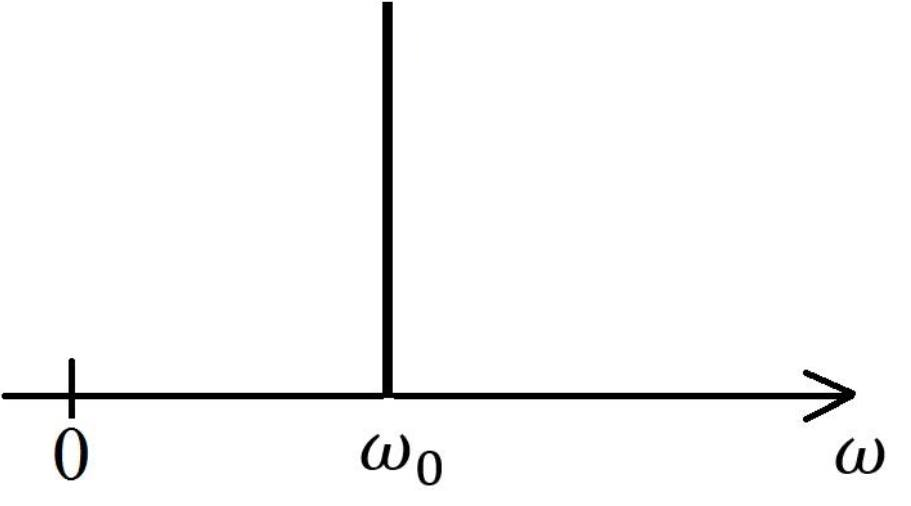
\includegraphics[width=0.8\textwidth]{USPSC-img/sharp_line.png}
		\vspace{5pt}
		\legend{Absorption or emission spectrum without line-broadening mechanisms so that we can assume the line shape $ g(\omega) = \delta(\omega - \omega_0) $.}
		\label{fig:shap-spectral-line}
	\end{subfigure}
	\hfill
	\begin{subfigure}[t]{0.45\textwidth}
		\centering
		\subcaption{Broadened spectral line}
		\vspace{8pt}
		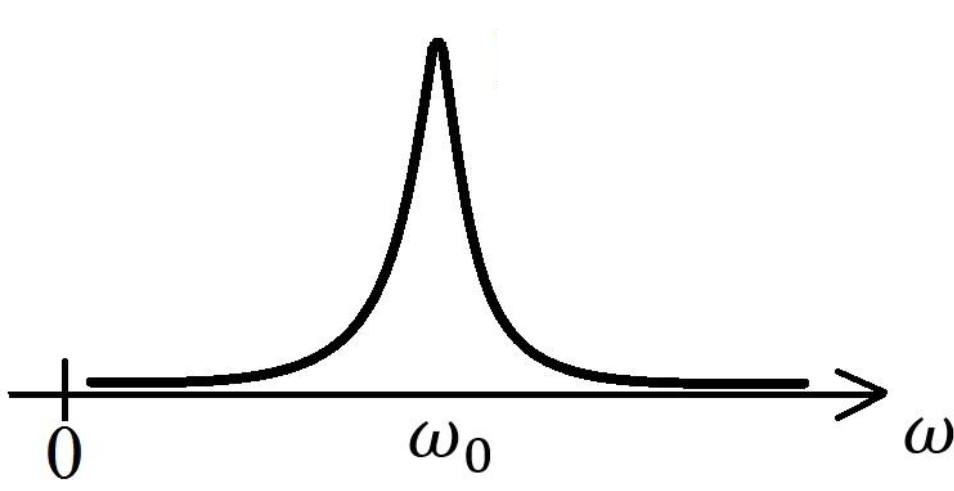
\includegraphics[width=0.8\textwidth]{USPSC-img/broadened_line.png}
		\vspace{5pt}
		\legend{Absorption or emission spectrum taking line-broadening mechanisms into account.}
		\label{fig:broadened-spectral-line}
	\end{subfigure}

	\legend{Source: \cite{valverde2016mecanismos}}
	\vspace{-20pt}
	\label{fig:spectral-broadening}
\end{figure}

We can take these mechanisms into account by introducing the normalized function $ g $ called \textbf{line shape function}. This function can be understood as the probability of absorbing or emitting a photon with frequency between $ \omega $ and $ \omega + d\omega $. A common $ g $ function in atomic spectroscopy is the \textit{Lorentzian}\footnote{Some authors define this distribution as a function of the frequency $ \nu $ instead of the angular frequency $ \omega = 2\pi\nu $.} (Cauchy distribution) given by
\begin{equation}
	g(\omega) = \frac{\Gamma'}{2\pi} \frac{1}{(\omega - \omega_0)^2 + (\Gamma' / 2)^2}\ \ \textrm{or}\ \ g(\Delta) = \frac{\Gamma'}{2\pi} \frac{1}{\Delta^2 + (\Gamma' / 2)^2},
\end{equation}
where $ \Delta = \omega - \omega_0 $ is the \textbf{detuning} and $ \Gamma' $ is the full width at half maximum (FWHM) also known as \textbf{spectral linewidth}. The main spectral linewidth is $ \Gamma' = A $, which is related to the energy-time uncertainty principle. Thus,
\begin{equation}
	g(\omega) = \frac{A}{2\pi} \frac{1}{(\omega - \omega_0)^2 + (A / 2)^2}\ \ \textrm{or}\ \ g(\Delta) = \frac{A}{2\pi} \frac{1}{\Delta^2 + (A / 2)^2}.
	\label{eq:line-shape-simplest-case}
\end{equation}

The probability distribution of finding an atom in the excited state taking the line shape function into account is given by
\begin{equation}
	\rho(t) = (1 - 2P) B \int_{0}^{\infty} u(\omega) g(\omega) d\omega - A P.
	\label{eq:distribution-upper-level-line-shape}
\end{equation}
For a broadband electromagnetic field, which means $ u(\omega) $ much broader than $ g(\omega) $, the equations (\ref{eq:distribution-upper-level-line-shape}) and (\ref{eq:distribution-upper-level}) are equivalent because
\begin{equation}
	\int_{0}^{\infty} u(\omega) g(\omega) d\omega \simeq u(\omega_0) \int_{0}^{\infty} g(\omega) d\omega = u(\omega_0).
	\label{eq:broadband-light-relation}
\end{equation}

%
%-----------------------------------
\subsection{Monochromatic light field}
%-----------------------------------
%

Let us consider a monochromatic electromagnetic field with frequency $ \omega $ interacting with an atom initially in the ground state. In the case, the spectral intensity $ I(\omega) $ and the spectral density energy $ u(\omega) $ of the light field is $ I(\omega') = c u(\omega') = I_0 \delta(\omega' - \omega) $, where $ I_0 $ is the total intensity and $ \delta(x) $ is the Dirac delta. Thus,
\begin{equation}
	\int_{0}^{\infty} u(\omega') g(\omega') d\omega' = \frac{I_0}{c} \int_{0}^{\infty} g(\omega') \delta(\omega' - \omega) d\omega' = \frac{I_0}{c} g(\omega).
	\label{eq:line-broadening-monochromatic-radiation}
\end{equation}
From equation (\ref{eq:distribution-upper-level-line-shape}) and (\ref{eq:line-broadening-monochromatic-radiation}), we obtain
\begin{equation}
	\rho(t) = (1 - 2P) \frac{\alpha(\omega)}{2} - A P,
	\label{eq:distribution-excited-state-monochromatic-light}
\end{equation}
where $ \alpha(\omega) = 2B(I_0 / c)g(\omega) $ is the \textbf{pumping rate}. The stationary solution of (\ref{eq:distribution-excited-state-monochromatic-light}) is given by
\begin{equation}
	P(t) = \frac{1 / 2}{1 + A / \alpha(\omega)} = \frac{1}{2} \frac{s(\omega)}{1 + s(\omega)},
	\label{eq:probability-excited-state-monochromatic-light}
\end{equation}
where $ s(\omega) = \alpha(\omega) / A $ is the \textbf{saturation parameter}, which defines the balance between pumping and relaxation. From equation (\ref{eq:relation-A-B}), we have
\begin{equation}
	s(\omega) = \frac{2\pi^2 c^2}{\hbar \omega_0^3} I_0 g(\omega) = \frac{2\lambda_0^3}{h c} I_0 g(\omega) = \frac{I_0}{I_s} \frac{g(\omega)}{g(\omega_0)},\ \ \textrm{where}\ \ I_s \equiv \frac{\hbar \omega_0^3}{2\pi^2 c^2 g(\omega_0)} .
	\label{eq:saturation-parameter-ERE}
\end{equation}
The intensity $ I_s $ is called \textbf{saturation intensity}. When $ s(\omega) \gg 1 $, stimulated processes are more significant than spontaneous emission, implying the saturation $ P \longrightarrow 1/2 $. When $ s(\omega) \ll 1 $, relaxation processes are predominant. In this case, the atom will certainly decay to the ground state, $ P \longrightarrow 0 $.

%
%-----------------------------------
\subsection{Absorption cross section}
\label{sec:absorption-cross-section}
%-----------------------------------
%

\begin{wrapfigure}{l}{0.45\textwidth}
	\centering
	\caption{Absorption Cross Section}
	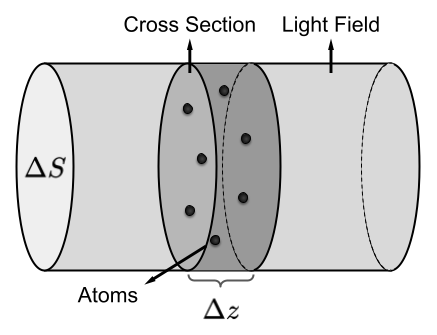
\includegraphics[width=0.43\textwidth]{USPSC-img/cross_section_scheme.png}
	\legend{Dilute atomic gas interacting with a electromagnetic radiation in a slab of thickness $ \Delta z $ and volume $ \Delta S \Delta z $. \\ Source: Author}
	\vspace{-15pt}
	\label{fig:absorption-cross-section}
\end{wrapfigure}

In atomic spectroscopic, it is common to analyze the attenuated or amplified light beam which passes through an atomic medium \cite{reinaudi2007strong, smith2011absorption, shu2004absorption}. Let us consider an electromagnetic beam with total spectral intensity $ I(\omega, z) $ propagating in the z-direction. This radiation passes through an atomic ensemble with $ n_1 $ atoms per volume in the ground state and $ n_2 $ atoms per volume in the excited state (figure \ref{fig:absorption-cross-section}), being attenuated or amplified in each slab of thickness $ \Delta z $ due to stimulated absorption. Its spectral intensity will be reduced by a fraction of $ n_1 \sigma(\omega) \Delta z $, where $ \sigma(\omega) $, known as \textbf{absorption cross-section}\footnote{The absorption cross-section is expressed in units of area}, is related to the probability that an atom will absorb an photon with angular frequency between $ \omega $ and $ \omega + d\omega $ from the light field on the section where this light passes on. Therefore, the lost spectral intensity is given $ \Delta I / I = - N \sigma \Delta z $ and then
\begin{equation}
	\frac{dI}{dz}(\omega, z) = - n_1 \sigma(\omega) I(\omega, z).
	\label{eq:lost-spectral-intensity}
\end{equation}
Besides the light attenuation due to stimulated absorption, there are also gain due to stimulated emission. Spontaneous emission does not contribute to the gain since the emitted light is isotropic. In this case, the light field will be amplified in each slab, increasing its intensity by a fraction of $ n_2 \sigma(\omega) \Delta z $. Here, the quantity $ \sigma $ gives the probability of emitting light stimulately. The absorption cross-section and the emission cross-section are the same since the absorption rate equals the emission rate ($ B_{12} = B_{21} $ when $ g_1 = g_2 $). Therefore, the light gain is given by
\begin{equation}
	\frac{dI}{dz}(\omega, z) = n_2 \sigma(\omega) I(\omega, z).
	\label{eq:spectral-density-power}
\end{equation}
From equations (\ref{eq:lost-spectral-intensity}) and (\ref{eq:spectral-density-power}), we obtain
\begin{equation}
	\frac{dI}{dz}(\omega, z) = - (n_1 - n_2) \sigma(\omega) I(\omega, z)
	\label{eq:net-spectral-density-power}
\end{equation}
where $ (dI / dz) \Delta S \Delta z $ is equivalent to the net spectral power (power per unit of frequency) gained or lost by the radiation in a slab of thickness $ \Delta z $ due to stimulated processes\footnote{Spontaneous emitted light does not come back to the radiation field, since it is isotropic.}. It is convenient to define a \textbf{net absorption cross-section} as 
\begin{equation}
	\sigma_{abs}(\omega) = \frac{n_1 - n_2}{n} \sigma(\omega) = (1 - 2P)\sigma(\omega),
	\label{eq:net-absorption-cross-section}
\end{equation}
where $ n = n_1 + n_2 $ is the total density number and $ P $ is the probability of finding an atom in the excited state. This cross-section is associated with the probability of an atom attenuating or amplifying an incident light due to stimulated processes. Solving the differential equation (\ref{eq:net-spectral-density-power}), we obtain
\begin{equation}
	I(\omega, z) = e^{-n\sigma_{abs}(\omega)t}I(\omega, 0),
	\label{eq:Beer-Lambert-law}
\end{equation}
In the regime of weak excitation such that $ n_2 \ll n_1 $, the total number density is approximately the number density of the atoms in the ground state $ n \simeq n_1 $ and then $ \sigma_{abs}(\omega) \simeq \sigma(\omega) $.

Let us assume a \textit{monochromatic} radiation whose frequency is $ \omega $ such that $  I(\omega', z) = I_0(z) \delta(\omega' - \omega) $ and $ u(\omega', z) = I(\omega', z) / c $. In this case, integrating equation (\ref{eq:net-spectral-density-power}) over all frequencies, we obtain the total power per unit of volume gained or lost by the radiation
\begin{equation}
	\frac{d I_0}{dz}(z) = -n\sigma_{abs}(\omega)I_0(z)\ \ \Rightarrow\ \ I_0(z) = I_0(0) e^{- n\sigma_{abs}(\omega)z}.
	\label{eq:Beer-Lambert-law-total-power}
\end{equation}
In the steady state, $ (dI_0/dz) $ equals the total power per unit of volume lost by spontaneous emission. Then, from equation (\ref{eq:Beer-Lambert-law-total-power}), we have
\begin{gather}
	n\sigma_{abs}(\omega) I_0 = A n_2 \hbar \int_0^{\infty} \omega g(\omega)d\omega.
	\label{eq:cross-section-expression}
\end{gather}
Since $ \omega_0 $ is much greater than the FWHM of $ g(\omega) $\footnote{The line shape function must be normalized over $ 0 $ to $ \infty $, which demands that the peak frequency $ \omega_0 $ of $ g(\omega) $ must be much greater than its FWHM.}, thus
\begin{equation}
	\int_0^{\infty} \omega g(\omega)d\omega \simeq \omega_0.
\end{equation}
Then, from equation (\ref{eq:cross-section-expression}), we have
\begin{equation}
	n \sigma_{abs}(\omega) I_0 = A n_2 \hbar \omega_0\ \Rightarrow\ \sigma_{abs}(\omega) = \frac{\hbar \omega_0}{I_0} A P,
	\label{eq:net-absorption-cross-section}
\end{equation}
where $ P = n_2 / n $. Therefore, in the steady state, the \textit{net absorption cross-section} can be understood as an area on which the photon flux of the incident beam passes through times the rate $ \Gamma P $ at which an atom scatters photons by spontaneous emission, i.e. the decay rate $ \Gamma $ times the probability of finding an atom in the excited state. From equations (\ref{eq:probability-excited-state-monochromatic-light}), (\ref{eq:saturation-parameter-ERE}), and (\ref{eq:net-absorption-cross-section}), we obtain
\begin{gather}
	\sigma(\omega) = \frac{\hbar \omega_0}{I_0} \frac{A}{2} s(\omega) = \overbrace{\frac{\hbar \omega_0}{I_s} \frac{A}{2}}^{\sigma_0} \frac{g(\omega)}{g(\omega_0)} = \sigma_0 \frac{g(\omega)}{g(\omega_0)}\ \ \textrm{and}
	\label{eq:absorption-cross-section-2}
	\\
	\sigma_{abs}(\omega) = \frac{\hbar \omega_0}{I_0} \frac{A}{2} \frac{s(\omega)}{1 + s(\omega)} = \sigma(\omega) \frac{1}{1 + s(\omega)},
	\label{eq:net-absorption-cross-section-2}
\end{gather}
where $ \sigma_0 \equiv \sigma(\omega_0) $ is the \textit{resonant absorption cross-section} which only depends on the properties of the atom ($ I_s$, $ \omega_0 $, and $ A $).




%-----------------------------------
%


% Semiclassical Approach
%-----------------------------------
%
%--- 
%-----------------------------------
\section{Semiclassical approach}
\label{sec:semiclassical-approach}
%-----------------------------------
%--- 
%

In the previous section, we consider phenomenological rate equations to study two-level atomic transitions. This approach does not contemplate coherence effects nor a fundamental understanding of line broadening mechanisms. In a first attempt, we can take the coherence effects into account assuming the interaction between a classical light field (electromagnetic waves) and an atom whose internal states are described by a quantum state vector $ \ket{\psi} $. Indeed, this is a proper treatment as long as we are only interested in stimulated processes. However, spontaneous emission comes from the interaction between atom and the vacuum modes of the quantized electromagnetic field, an incoherent relaxation process. Therefore, a single state vector is not sufficient to analyze an atom under both stimulated and spontaneous processes since such system is under decoherence. A proper description comes through the density operator, which describes a statistical mixture of quantum states. This approach allows us to study the system time evolution taking both coherent and incoherent processes into account through a master equation. In this section, we shall introduce the density operator formalism to investigate atom-light interaction.

%
%-----------------------------------
\subsection{The density operator}
\label{sec:density-operator}
%-----------------------------------
%

The density operator represents an \textbf{ensemble} of identical systems in different quantum states. Let us consider a system which can be found in a quantum state $ \ket{\psi_k} $ with probability $ P_{k} $. This system is represented by the following density operator
\begin{equation}
	\hat{\rho} \equiv \sum_{k} P_{k} \ketbra{\psi_k}{\psi_k}\ \ \ \ \textrm{so that}\ \ \ \sum_k P_k = 1.
\end{equation}
When the system is described by a single state vector $ \ket{\psi} $, which means $ \hat{\rho} = \ketbra{\psi}{\psi} $, it is said to be in a \textbf{pure state}, otherwise it is said to be in a \textbf{mixed state}.

Let us consider the orthonormal basis $ \{\ket{n} : n \in \{1, 2, \cdots, N\}\} $ on which it is possible to represent the states $ \{\ket{\psi_k}\} $ and the density operator $ \hat{\rho} $ as
\begin{gather}
	\ket{\psi_k} = \sum_{n = 1}^{N} |c_{k,n}|e^{\phi_{k,n}} \ket{n},\ \ 
	\hat{\rho} = \left[ 
	\begin{matrix}
		\rho_{1,1} & \cdots & \rho_{1,N} \\
		\vdots & \ddots & \vdots \\
		\rho_{N,1} & \cdots & \rho_{N,N}
	\end{matrix} \right], \\
	\textrm{where}\ \ \ \rho_{m,n} = \braket{m|\hat{\rho}|n}\ \ \textrm{(matrix elements),}
\end{gather}
being $ \rho $ the \textbf{density matrix} and $ c_{k,n} = |c_{k,n}|e^{\phi_{k,n}} $. From now on, we shall assuming the abuse of notation $ \hat{\rho} = \rho $ in order to make the definion of a density operator easy by using its matrix represantion. The probability of finding a state $ \ket{n} $ in a given state vector $ \ket{\psi_k} $ is $ P_k |c_{k,n}|^2 $. Then the probability of finding the state $ \ket{n} $ in any state vector is
\begin{equation}
	\sum_{k} P_k |c_{k,n}|^2 = \sum_{k} P_k \underbrace{\braket{n|\psi_k}}_{c_{k,n}}\underbrace{\braket{\psi_k|n}}_{c_{k,n}^*} = \bra{n} \left( \sum_k P_k \ketbra{\psi_k}{\psi_k} \right) \ket{n} = \braket{n|\hat{\rho}|n} = \rho_{n,n}.
\end{equation}
Therefore, the diagonal terms, also referred as \textbf{populations}, give the probability of measuring the system in some state $ \ket{n} $, which implies
\begin{equation}
	\Tr[\rho] = \sum_{n = 1}^{N} \braket{n|\hat{\rho}|n} = \sum_{n = 1}^{N} \rho_{n,n} = 1,
\end{equation} 
where $ Tr[\hat{\rho}] $ is the \textbf{trace} of the operator $ \hat{\rho} $. This operation is independent of the basis since it is invariant with respect to any unitary transformation. Moreover, the trace is also invariant under cyclic permutation of the product so that
\begin{equation}
	\Tr[\hat{A}\hat{B}\hat{C}] = \Tr[\hat{B}\hat{C}\hat{A}] = \Tr[\hat{C}\hat{A}\hat{B}].
\end{equation}
The off-diagonal terms are called \textbf{coherences}. They give information about the relative phase of different components. Let us consider a pure state so that
\begin{align}
	\rho_{m,n} &= \bra{m}(\ketbra{\psi}{\psi})\ket{n} = \bra{m}\left(\sum_{p} |c_p|e^{i\phi_p} \ket{p}\right)\left(\sum_{q} |c_q|e^{- i \phi_{q}} \bra{q}\right)\ket{n} \\
	&= \sum_{p,q} |c_p c_q |e^{i(\phi_p - \phi_q)} \braket{m|p} \braket{q|n} = |c_m c_n| e^{i(\phi_m - \phi_n)}
\end{align}
For mixed systems, the coherences will be the sum of complex numbers corresponding to different states $ \ket{\psi_k} $. Furthermore, it is possible to check whether a system is pure or mixed evaluating the quantity $ \Tr[\hat{\rho}^2] $. For a pure state $ \hat{\rho}_{pure} = \ket{\psi}\bra{\psi} $, we have 
\begin{equation}
	\hat{\rho}_{pure}^2 = \ket{\psi}\braket{\psi|\psi}\bra{\psi} = \ketbra{\psi}{\psi} = \hat{\rho}_{pure} \Rightarrow \Tr[\hat{\rho}_{pure}^2] = \Tr[\hat{\rho}_{pure}] = 1.
\end{equation}
Indeed, $ \hat{\rho}_{pure}^n = \hat{\rho}_{pure} $ for any pure state, being $ n $ a non-negative integer. To study the case of a mixed state defined by the density operator $ \hat{\rho}_{mixed} $, let us assume a basis where the matrix $ \rho_{mixed} $ is diagonal so that
\begin{equation}
	\Tr[\rho_{mixed}^2] = \sum_n (\rho_{n,n})^2 \leq \sum_n \rho_{n,n} = 1,
\end{equation}
since $ 0 \leq \rho_{n,n} \leq 1 $. A diagonal pure state has only a single non-zero element, whereas a diagonal mixed state necessarily has more then one non-zero element. Hence, being the trace operation independent of the basis, for a mixed state we always have
\begin{equation}
	\Tr[\hat{\rho}_{mixed}^2] < 1.
\end{equation}

We can also compute expectation values using the trace operation. Let us consider an observable $ \hat{A} $ whose matrix elements are $ A_{m,n} = \braket{m|\hat{A}|n} $. The expectation value $ \braket{\hat{A}} $ is expressed by
\begin{equation}
	\braket{\hat{A}} = \sum_{k} P_k \braket{\psi_k|\hat{A}|\psi_k}.
\end{equation}
On the other side,
\begin{gather}
	\hat{\rho}\hat{A} = \sum_{k} P_k \ketbra{\psi_k}{\psi_k}\hat{A} \Rightarrow \braket{n|\hat{\rho}\hat{A}|n} = \sum_{k} P_k \braket{\psi_k|\hat{A}|n} \braket{n|\psi_k} \Rightarrow \\
	\Rightarrow \Tr[\hat{\rho}\hat{A}] = \sum_{n} \braket{n|\hat{\rho}\hat{A}|n} = \sum_{k} P_k \bra{\psi_k} \hat{A} \underbrace{\left( \sum_{n = 1}^{N} \ketbra{n}{n} \right)}_{\mathbb{I}} \ket{\psi_k} = \sum_{k} P_k \braket{\psi_k|\hat{A}|\psi_k} \\
	\therefore \Tr[\hat{\rho}\hat{A}] = \sum_{k} P_k \braket{\psi_k|\hat{A}|\psi_k} = \braket{\hat{A}}.
	\label{eq:trace-average}
\end{gather}
Therefore, the ensemble average of any observable $ \hat{A} $ can be calculated from the diagonal elements of the operator matrix $ \hat{\rho}\hat{A} $.

The density operator formalism is also great to manage \textbf{composite system}. Let us consider a system $ A $ defined by the density operator $ \hat{\rho}_A $ and the Hilbert space $ \mathcal{H}_{A} $, and a system $ B $ represented by the density operator $ \hat{\rho}_B $ and the Hilbert space $ \mathcal{H}_B $. The total system, which take A and B into account, is described by the density operator $ \hat{\rho}_{AB} $ and the Hilbert Space $ \mathcal{H}_A \otimes \mathcal{H}_B $. The operator $ \hat{\rho_A} $ and $ \hat{\rho_B} $ can be seen as \textbf{reduced density matrices}, which can be derived from $ \hat{\rho}_{AB} $ through the \textbf{partial trace operation},
\begin{equation}
	\hat{\rho}_A = \Tr_{B} [\hat{\rho}_{AB}]\ \ \ \textrm{and}\ \ \ \hat{\rho}_B = \Tr_A [\hat{\rho}_{AB}].
\end{equation}

Let us consider a pure state $ \ket{\psi_{AB}} $ of both system $ A $ and $ B $ given by
\begin{equation}
	\ket{\psi_{AB}} = \sum_{m,n} c_{m,n} \ket{m} \otimes \ket{n},\ \ \textrm{where}\ \ \sum_{m,n} |c_{m,n}| = 1.
	\label{eq:ket-A-B}
\end{equation}
If the systems are \textit{independent}, we can associate a state $ \ket{\psi_A} = \sum a_m \ket{m} $ to the system $ A $ and $ \ket{\psi_B} = \sum b_n \ket{n} $ to the system $ B $ so that
\begin{equation}
	\ket{\psi_{AB}} = \ket{\psi_A} \otimes \ket{\psi_B} = \left( \sum_m a_m \ket{m} \right) \otimes \left( \sum_n b_n \ket{n} \right) = \sum_{m,n} a_m b_n \ket{m} \otimes \ket{n}.
	\label{eq:ket-A-B-independent-systems}
\end{equation}
From equations (\ref{eq:ket-A-B}) and (\ref{eq:ket-A-B-independent-systems}), we obtain $ c_{m,n} = a_m b_n $. Then, the density operator $ \hat{\rho}_{AB} $ is given by
\begin{align}
	\hat{\rho}_{AB} &= \ketbra{\psi_{AB}}{\psi_{AB}} = \sum_{m,n} \sum_{m',n'} a_{m} a_{m'} b_{n} b_{n'} \ketbra{m}{m'} \otimes \ketbra{n}{n'} = \nonumber\\
	&= \left( \sum_{m,m'} a_m a_m' \ketbra{m}{m'} \right) \otimes \left( \sum_{n,n'} b_n b_n' \ketbra{n}{n'} \right) = \nonumber \\ 
	&= \ketbra{\psi_A}{\psi_A} \otimes \ketbra{\psi_B}{\psi_B} = \hat{\rho}_a \otimes \hat{\rho}_B.
\end{align}
Therefore, when two systems $ A $ and $ B $ are \textbf{uncorrelated} or \textit{independent}, we can write the density operator of both systems as a tensor product between the density operator of the system $A $ and the density operator of the system $ B $,
\begin{equation}
	\hat{\rho}_{AB} = \hat{\rho}_A \otimes \hat{\rho}_B.
\end{equation}


%
%-----------------------------------
\subsection{Two-level system and the Bloch sphere}
\label{sec:two-level-system-Bloch-sphere}
%-----------------------------------
%

Let us consider a system composed of only two quantum states $ \ket{1} $ and $ \ket{2} $, in which $ \ket{1} $ is the \textit{ground state} and $ \ket{2} $ is the excited state. An arbitrary two-dimensional density operator can be represent as
\begin{equation}
	\hat{\rho} = \left[ \begin{matrix} \rho_{1, 1} & \rho_{1, 2} \\ \rho_{2, 1} & \rho_{2, 2}\end{matrix}\right],
	\label{eq:density-operator-two-level-system}
\end{equation}
where $ \rho_{i,j} = \braket{i|\hat{\rho}|j} $. In the previous section \ref{sec:density-operator}, we saw that the diagonal terms represent probabilities so that $ \rho_{1,1} + \rho_{2,2} = 1 $, being $\rho_{1,1} $ and $ \rho_{2,2} $ real values. Also, $ \hat{\rho} $ must be hermitian and therefore $ \rho_{1,2} = (\rho_{2,1})^* $. The density matrix (\ref{eq:density-operator-two-level-system}) is represented on the basis
\begin{equation}
	\left\{\left[ \begin{matrix} 1 & 0 \\ 0 & 0 \end{matrix} \right],\ \left[ \begin{matrix} 0 & 1 \\ 0 & 0 \end{matrix} \right],\ \left[ \begin{matrix} 0 & 0 \\ 1 & 0 \end{matrix} \right],\ \left[ \begin{matrix} 0 & 0 \\ 0 & 1 \end{matrix} \right] \right\}.
\end{equation}
Another convenient basis is the \textbf{Pauli matrices basis},
\begin{equation}
	\left\{\sigma_x = \left[ \begin{matrix} 0 & 1 \\ 1 & 0 \end{matrix} \right],\ \sigma_y = \left[ \begin{matrix} 0 & -i \\ i & 0 \end{matrix} \right],\ \sigma_z = \left[ \begin{matrix} 1 & 0 \\ 0 & -1 \end{matrix} \right],\ \mathbb{I}_2 = \left[ \begin{matrix} 1 & 0 \\ 0 & 1 \end{matrix} \right] \right\},
\end{equation}
where $ \sigma_x $, $ \sigma_y $, and $ \sigma_z $ are the \textit{Pauli matrices}. An arbitrary density matrix on this basis is written as\footnote{For an arbitrary operator, we should have four coefficients $ [\hat{A}] = a_0 \mathbb{I} + a_1 \sigma_x + a_2 \sigma_y + a_3 \sigma_z $. In the case of the density matrix, we must have $ a_0 = 1/2 $ due to the property $ \Tr[\hat{\rho}] = 1 $.}
\begin{gather}
	\hat{\rho} = \frac{1}{2}(\mathbb{I}_2 + \mathbf{a} \cdot \vec{\sigma}) = \frac{1}{2}\left[ \begin{matrix} 1 + a_3 & a_1 - ia_2 \\ a_1 + i a_2 & 1 - a_3 \end{matrix} \right], 
	\label{eq:density-matrix-on-Pauli-basis}
	\\
	\textrm{where}\ \ \vec{\sigma} = \left[ \begin{matrix} \sigma_x \\ \sigma_y \\ \sigma_z \end{matrix} \right]\ \ \textrm{and}\ \ \mathbf{a} = \left[ \begin{matrix} a_1 \\ a_2 \\ a_3 \end{matrix} \right] \textrm{(\textbf{Bloch vector})}.
	\label{eq:Bloch-vector}
\end{gather}
In this representation, its eigenvalues are $ (1 \pm |\mathbf{a}|)/2$. Since they are probabilities, we must have $ 0 \leq (1 \pm |\mathbf{a}|)/2 \leq 1 \Rightarrow |\mathbf{a}| \leq 1 $. For the same reason, the diagonal terms, and then $ a_3 $, must be positive values. Furthermore, $ \hat{\rho} = \hat{\rho}^{\dagger} $, which implies $ a_1 = a_1^* $ and $ a_2 = a_2^* $. Hence, $ \mathbf{a} $ is a real vector. Comparing with the density matrix (\ref{eq:density-operator-two-level-system}), we have $ a_3 = \rho_{1,1} - \rho_{2,2} = p $ and $ (a_1 + i a_2) / 2 = \rho_{2,1} = q $, where $ p $ is known as \textbf{population inversion} and $ q $ is the \textit{coherence}. Then, the Bloch vector and the density matrix can be written as
\begin{equation}
	\mathbf{a} = \left[ \begin{matrix} 2\Re[q] \\ 2\Im[q] \\ p \end{matrix} \right] = \left[ \begin{matrix} q + q^* \\ i(q^* - q) \\ p \end{matrix} \right]\ \ \textrm{and}\ \ \hat{\rho} = \left[ \begin{matrix} (1 + p)/2 & q^{*} \\ q & (1 - p)/2 \end{matrix} \right].
	\label{eq:density-matrix-two-level-system}
\end{equation}
Taking the property $ |\mathbf{a}| \leq 1 $ into account, we can represent the Bloch vector in a ball of unitary radius known as \textbf{Bloch sphere} (although it is a ball, not a sphere) illustrated in figure \ref{fig:Bloch-sphere}. The axes are given by $x = 2\Re[q]$, $ y = 2\Im[q] $, and $ z = p $. When $ \hat{\rho} $ represent a pure state, we have
\begin{equation}
	\Tr[\hat{\rho}^2] = 1 \Rightarrow \frac{1}{2}(1 + |\mathbf{a}|^2) = 1 \Rightarrow |\mathbf{a}|^2 = 1.
\end{equation}
Therefore, the surface of the Bloch sphere represents all the pure states, whereas the inside corresponds to all the mixed states.

\noindent
\begin{minipage}{\textwidth}
	\begin{wrapfigure}{l}{0.45\textwidth}
		\centering
		\vspace{-10pt}
		\caption{Bloch sphere.}
		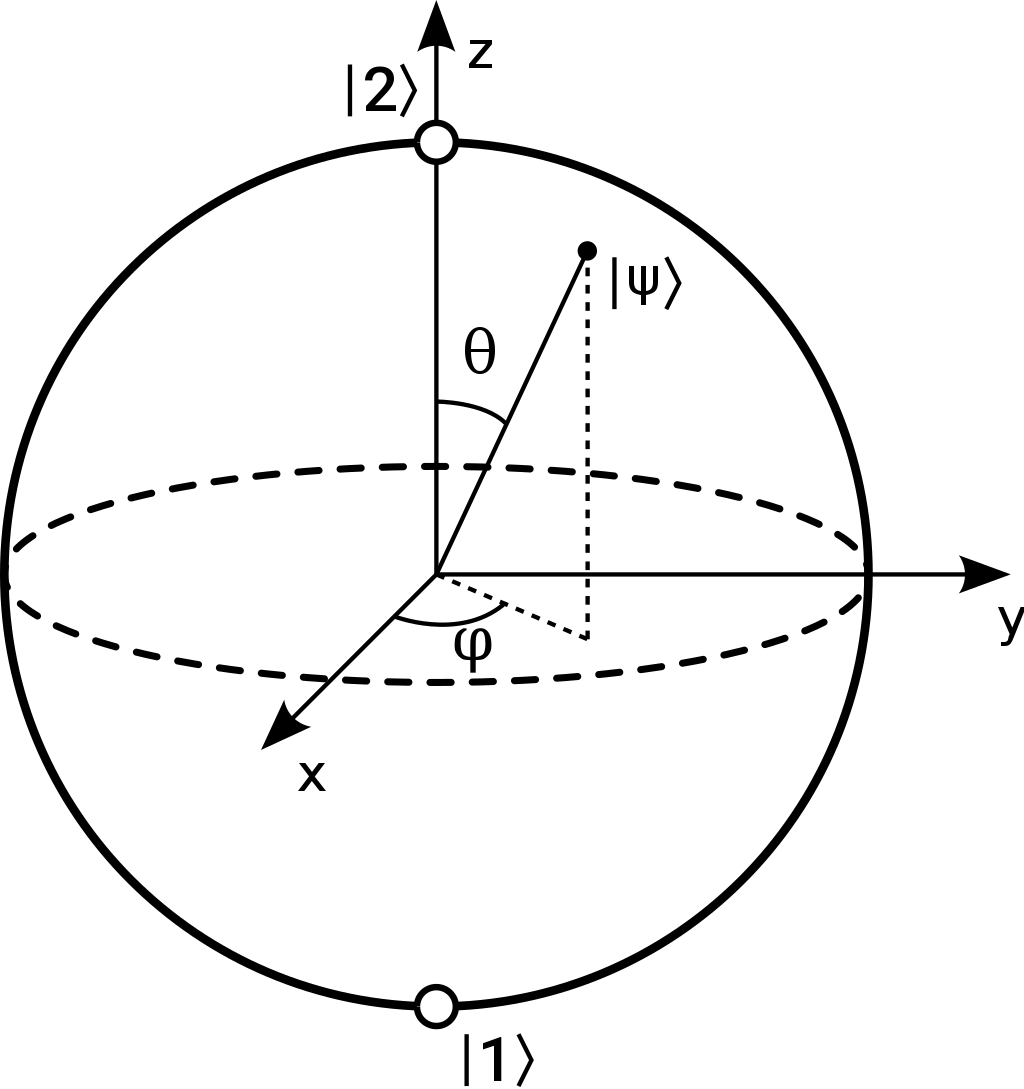
\includegraphics[width=0.35\textwidth]{USPSC-img/Bloch_sphere.png}
		\legend{Bloch sphere for a pure state given by \\ $ \ket{\psi} = \sin(\theta/2) \ket{1} + e^{i\phi} \cos(\theta/2) \ket{2} $. \\ Source: Author}
		\label{fig:Bloch-sphere}
		\vspace{-5pt}
	\end{wrapfigure}
	Let us consider a pure state $ \ket{\psi} = c_1\ket{1} + c_2\ket{2} $. Since a global phase is not measurable, we can assume $ \ket{\psi} = c_1 \ket{1} + c_2 e^{i\phi} \ket{2} $ where $ \phi $ is the phase difference between $ \ket{1} $ and $ \ket{2} $, and both $ c_1 $ and $ c_2 $ are real values. Moreover, $ c_1^2 + c_2^2 = 1 $, which allows us to associate $ c_1 $ and $ c_2 $ with a unique value $ \theta $ considering $ c_1 = \sin{(\theta/2)} $ and $ c_2 = \cos{(\theta/2)} $. Even though the value of $ \theta $ is not unique to represent $ c_1 $ and $ c_2 $, the point $ (\theta, \phi) $ is unique to represent $ \ket{\psi} $. Thus, a density operator $ \hat{\rho} = \ketbra{\psi}{\psi} $ of a pure state can be written as
	\begin{align}
		\hat{\rho} &= \sin^2(\theta/2) \ketbra{1}{1} + \cos^2(\theta/2) \ketbra{2}{2} + \nonumber 
		\\
		&+ \frac{1}{2}e^{-i\phi}\sin\theta \ketbra{1}{2} + \frac{1}{2}e^{i\phi}\sin\theta \ketbra{2}{1},
	\end{align}
\end{minipage}

\begin{equation}
	\hat{\rho} = \left[ \begin{matrix} \sin^2(\theta/2) & \frac{1}{2}e^{-i\phi}\sin\theta \\ \frac{1}{2}e^{i\phi}\sin\theta & \cos^2(\theta/2) \end{matrix} \right].
	\label{eq:density-matrix-pure-state-spherical-coordinates}
\end{equation}
From equations (\ref{eq:density-matrix-on-Pauli-basis}) and (\ref{eq:density-matrix-pure-state-spherical-coordinates}), we obtain the following Bloch vector
\begin{equation}
	\mathbf{a} = (\cos\phi \sin\theta, \sin\phi \sin\theta, \cos\theta),
\end{equation}
in which $ (\phi, \theta) $ are \textit{spherical coordinates} represented in figure \ref{fig:Bloch-sphere}.

%
%-----------------------------------
\subsection{Liouville equation}
\label{sec:Liouville-equations}
%-----------------------------------
%

The time evolution of a state vector $ \ket{\psi} $ is given by the Schrodinger equation $ \hat{H} \ket{\psi} = i \hbar \partial_t \ket{\psi} $, where $ \hat{H} $ is the Hamiltonian of the system. Thereby, the time evolution of $ \hat{\rho} $ is given by
\begin{align}
	\partial_t \hat{\rho} &= \partial_t \left( \sum_{k} P_k \ketbra{\psi_k}{\psi_k} \right) = \sum_{k} P_k [(\partial_t \ket{\psi_k})\bra{\psi_k} + \ket{\psi_k}(\partial_t \bra{\psi_k})] = \\
	&= \frac{i}{\hbar} \sum_{k} P_k (\ketbra{\psi_k}{\psi_k} \hat{H} - \hat{H}\ketbra{\psi_k}{\psi_k}) = \hat{\rho}\hat{H} - \hat{H}\hat{\rho}
\end{align}
Therefore,
\begin{equation}
	\partial_t \hat{\rho} = \frac{i}{\hbar} [\hat{\rho}, \hat{H}],
	\label{eq:Liouville-equation}
\end{equation}
where the equation (\ref{eq:Liouville-equation}) is called \textbf{von Neumann equation} or \textbf{Liouville equation}. The commutator itself can be considered as a \textbf{superoperator} acting on the density operator,
\begin{equation}
	\mathcal{L}\hat{\rho}(t) \equiv - \frac{i}{\hbar} [\hat{H}, \hat{\rho}(t)],
	\label{eq:Liouville-superoperator}
\end{equation}
where $ \mathcal{L} $ is known as \textbf{Liouville superoperator}. We shall work with a Hamiltonian in the form $ \hat{H} = \hat{H}_0 + \hat{V}(t) $, where $ \hat{H}_0 $ is a time-independent part and $ \hat{V}(t) $ is a time-dependent term. In this case, it is convenient to define an unitary transformation given by $ \hat{U}(t) = e^{- i \hat{H}_0 t / \hbar} $ so that 
\begin{equation}
	\hat{\rho}'(t) = \hat{U}^{\dagger}(t)\hat{\rho}(t)\hat{U}(t).
	\label{eq:density-operator-interaction-picture}
\end{equation}
Calculating the time derivatives on both sides of (\ref{eq:density-operator-interaction-picture}) and assuming (\ref{eq:Liouville-equation}), we obtain
\begin{equation}
	\partial_t \hat{\rho}'(t) = - \frac{i}{\hbar} [\hat{V}(t), \hat{\rho}'(t)].
	\label{eq:von-Neumann-equation-interaction-picture}
\end{equation}
The equation (\ref{eq:von-Neumann-equation-interaction-picture}) is the \textbf{Liouville equation} in the \textbf{interaction picture}, which depends only on the time-dependent part.

The equation (\ref{eq:Liouville-equation}) is valid as long as there are only coherent effects on the system,  since these processes are represented by unitary time evolutions\footnote{An unitary time evolution is associated with a hermitian Hamiltonian so that $ \hat{U} = e^{-i \hat{H}t / \hbar} $.}. In the context of atom-light interaction when we assume an density operator associated with the atomic internal states, the Liouville equation only describes stimulated absorption and emission. However, spontaneous emission is a predominant process in MOTs, so it is mandatory to take it into account. In order to comply with that, we shall introduce the \textit{master equation} in section \ref{sec:master-equation}.

%
%-----------------------------------
\subsection{Master equation}
\label{sec:master-equation}
%-----------------------------------
%

Spontaneous emission comes from a coupling between an open quantum system, described by the density operator $ \hat{\rho}_S $, and the environment, represented by the density operator $ \hat{\rho}_E $. Moreover, the environment must have far more degrees of freedom than the system. In our case, the system can be understood as the atom and the environment as the vacuum modes of the quantized electromagnetic field. Let us consider a density operator $ \hat{\rho}_{SE} $ which represents jointly the system and the environment. Assuming a weak coupling in which the system performs a small perturbation to the environment, we can treat both independently so that
\begin{equation}
	\hat{\rho}_{SE} \approx \hat{\rho}_S \otimes \hat{\rho}_E.
	\label{eq:Born-approximation}
\end{equation}
The equation (\ref{eq:Born-approximation}) is known as the \textbf{Born approximation}. At first, both system and environment provoke mutual excitations, getting out of thermal equilibrium. After a while, both will reach equilibrium again through a relaxation process. Let us consider the relaxation times $ \tau_E $ and $ \tau_S $ of the environment and the system, respectively. Since the system causes small perturbation to the environment but the environment interacts strongly with the system, we can consider $ \tau_E \ll \tau_S $. This is known as \textbf{Markov approximation}. The equation of motion of $ \hat{\rho}_{SE} $ is given by the Liouville equation,
\begin{equation}
	i \hbar \partial_t \hat{\rho}_{SE} = [\hat{H}_{SE}, \hat{\rho}_{SE}].
	\label{eq:Liouville-equation-system-environment}
\end{equation}
Let us consider a multi-level system given by the basis $\{\ket{n}\}$. Taking the Born-Markov approximation into account, it is possible to derive an equation of motion for $ \hat{\rho}_S $ tracing out the environment in equation (\ref{eq:Liouville-equation-system-environment}). The resulting equation \cite{brasil2013simple}, known as \textbf{master equation} or \textbf{Lindblad equation}, is given by
\begin{gather}
	\partial_t \hat{\rho}_S = \frac{1}{i\hbar} [\hat{H}_S, \hat{\rho}_S] + \sum_{i,j} \frac{\Gamma_{ij}}{2}(2\hat{\sigma}_{ij}\hat{\rho}_{S}\hat{\sigma}_{ji} - \{\hat{\sigma}_{ji}\hat{\sigma}_{ij}, \hat{\rho}_{S}\}) = (\mathcal{L} + \mathcal{L}_{decay}) \hat{\rho}_S,
	\label{eq:Lindblad-equation}
	\\
	\mathcal{L}_{decay}\hat{\rho} = \sum_{i,j} \frac{\Gamma_{ij}}{2}(2\hat{\sigma}_{ij}\hat{\rho}_{S}\hat{\sigma}_{ji} - \{\hat{\sigma}_{ji}\hat{\sigma}_{ij}, \hat{\rho}_{S}\}),
	\label{eq:Lindblad-superoperator}
\end{gather}
where $ \hat{\sigma}_{ij} = \ketbra{i}{j} $, $ \mathcal{L}_{decay} $ is the \textbf{Lindblad superoperator}, $ \{\hat{A}, \hat{B}\} = \hat{A}\hat{B} + \hat{A}\hat{B}$ is the anticommutator, and $ \{\Gamma_{i,j}\} $ are rates, known as \textit{decay rates}, at which both populations and coherences vanish. The operators $ \hat{\sigma}_{i,j} $ and $ \hat{\sigma}_{j,i} = \hat{\sigma}_{i,j}^{\dagger} $ can be understood as \textit{lower} and \textit{upper operators} between the states $ \ket{i} $ and $ \ket{j} $ so that $ \hat{\sigma}_{i,j} \ket{j} = \ket{i} $ and $ \hat{\sigma}_{j,i} \ket{i} = \ket{j} $. The master equation results in the Liouville equation when $ \Gamma_{ij} \longrightarrow 0,\ \forall i,j $. Therefore, the difference between these equations is the decay term expressed by the superoperator $ \mathcal{L}_{decay} $ known as \textbf{Lindblad superoperator}.

Let us consider the case in which only $ \{\Gamma_{i,i} = \Gamma_i \} $ are non-zero. Then, the superoperator $ \mathcal{L}_{decay} $ can be written as
\begin{equation}
	\mathcal{L}_{decay} \hat{\rho} = - \frac{1}{2} \sum_{i} \Gamma_i \left( \sum_{j \neq i} \rho_{i,j} \ketbra{i}{j} + \sum_{k \neq i} \rho_{k,i} \ketbra{k}{i} \right),
	\label{eq:decay-superoperator-dephasing}
\end{equation}
where $ \rho_{i,j} \equiv \braket{i|\hat{\rho}|j} $. From equation (\ref{eq:decay-superoperator-dephasing}), it is possible to see that only the off-diagonal terms are affected by $ \mathcal{L}_{decay} $. Hence, only the coherences decay since they are associated with the off-diagonal terms. This process is known as \textbf{pure dephasing}. In the general case when $ \Gamma_{i,j} > 0 $ for $  i \neq j $, the populations also change over time, which is known as \textbf{relaxation}. Spontaneous emission is only responsible for \textit{relaxation} terms $ \{ \Gamma_{i,j},\ i \neq j,\ i  < j \} $, whereas the \textit{pure dephasing} terms $ \{ \Gamma_{i} \} $ are associated with \textbf{elastic collisions}. Furthermore, $\{ \Gamma_{i} \} $ are the rates at which the atoms collide between each other. We are concerned only with the regime of low temperatures in which collisions are negligible.
%-----------------------------------
%

% Two-level atom interacting with classical light field
%-----------------------------------
\input{USPSC-TA-Textual/Atom-Light-Interaction/two-level-atom.tex}
%-----------------------------------
%

% Line broadening mechanisms
%-----------------------------------
%%
%-----------------------------------
\section{Line-broadening mechanisms}
\label{sec:line-broadening-mechanisms}
%-----------------------------------
%

In section \ref{sec:spectral-broadening}, we introduce the \textit{line shape function} $ g(\omega) $, which gives the probability of either absorbing or emitting a photon with a frequency between $ \omega $ and $ \omega + d\omega $. This function is proportional to the \textit{absorption cross-section} $ \sigma(\omega) $ according equation (\ref{eq:absorption-cross-section-2}). Although the line shape function take spectral broadening into account, it is not directly proportional to both absorbing and fluorescence profiles, which are actually measured. Theses profiles are associated directly with the \textit{net absorption cross-section} $ \sigma_{abs} $ and the \textit{scattering cross-section} $ \sigma_{sc} $. From equations (\ref{eq:net-absorption-cross-section-3}) and (\ref{eq:scattering-cross-section}), we can see that the absorption profile is not a sharp line as discussed in section \ref{sec:spectral-broadening}. In the next sections, we shall discuss physical effects which can both broaden and shift the absorption/scattering cross-section profile. Overall, there are two types of line broadening mechanisms: 
\begin{itemize}
	\item \textbf{Homogeneous broadening:} all atoms in a medium are affected in the same way. In this case, we can add these line-broadening mechanisms in the optical Bloch equations so that it is valid for all atoms in the medium;

	\item \textbf{Inhomogeneous broadening:} each atom in a medium is individually affected. In this case, we can only described line-broadening mechanisms in the optical Bloch equations for individual atoms. Therefore, we can not generalize for all atoms in the medium.
\end{itemize}

%-----------------------------------
\subsection{Natural broadening}
\label{sec:natural-broadening}
%-----------------------------------

Let us assume an isolated atom initially in the excited state so that there is not an incident light beam ($ s_0 = 0 $). This atom will decay in an average time $ 1/\Gamma $. In other words, $ 1 / \Gamma $ is the average time for the system changes considerably. Therefore, due to the \textit{time-energy uncertainty principle}, there will be an energy uncertainty in the excited state given by
\begin{equation}
	\Delta E \geq \frac{\hbar}{2\Delta t} = \frac{\hbar\Gamma}{2}.
\end{equation}
\begin{figure}[!ht]
	\centering
	\vspace{0pt}
	\caption{Natural broadening}
	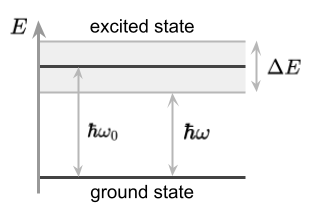
\includegraphics[width=0.4\textwidth]{USPSC-img/natural_broadening.png}
	\vspace{5pt}
	\legend{Energy uncertainty of a excited state whose lifetime is $ 1/\Gamma $. Due to the time-energy uncertainty principle, $ \Delta E \geq \hbar \Gamma / 2 $ and then a spontaneously emitted photon have a random energy $ \hbar \omega $ whose the average is $ \hbar \omega_0 $ and the uncertainty is greater than $ \hbar \Gamma / 2 $.\\ Source: Author}
	\vspace{-10pt}
	\label{fig:natural-broadening}
\end{figure}
Spontaneously emitted photons do not have a deterministic energy $ \hbar \omega_0 $ since the system does not have either, as illustrated in figure \ref{fig:natural-broadening}. This phenomena provokes a \textit{homogeneous} line-broadening known as \textbf{natural broadening} or \textbf{lifetime broadening}. The probability of spontaneously emitting a photon with frequency between $ \omega $ and $ \omega + d\omega $ is given by the line shape function $ g(\omega) $ and it is proportional to the absorption cross-section $ \sigma(\omega) $ according equations (\ref{eq:line-shape-function-2}) and (\ref{eq:absorption-cross-section-3}). From equation (\ref{eq:line-shape-function-2}), we have
\begin{equation}
	g(\Delta) = \frac{1}{\pi} \frac{\Gamma / 2}{\Delta^2 + (\Gamma / 2)^2}.
	\label{eq:line-shape-function-natural-broadening}
\end{equation}
The equation (\ref{eq:line-shape-function-natural-broadening}) is \textit{Lorentzian profile} whose FWHM, also known as \textit{linewidth}, is $ \Gamma $, which is in agreement to equation (\ref{eq:line-shape-simplest-case}) proposed in section \ref{sec:spectral-broadening}. Since $ \Gamma $ is associated with the natural broadening, it is also called \textbf{natural linewidth}. In the regime of weak excitation so that $ s_0 \ll 1 $, the absorption cross-section approximately equals the net absorption cross-section such that $ \sigma \simeq \sigma_{abs} $.
 
%-----------------------------------
\subsection{Power broadening}
\label{sec:power-broadening}
%-----------------------------------

In the presence of a light field so that $ s_0 > 0 $, the only spectral broadening is the natural broadening given by (\ref{eq:line-shape-function-natural-broadening}). However, the net absorption cross-section $ \sigma_{abs} $ does not equal the absorption cross-section $ \sigma $. According to equation (\ref{eq:net-absorption-cross-section-2}), there will be a decreasing by a factor of $ 1 + s(\omega) $, which causes a line-broadening illustrated in figure (\ref{fig:net-absorption-cross-section}). From equations (\ref{eq:net-absorption-cross-section-3}) and (\ref{eq:absorption-cross-section-3}), we have
\begin{gather}
	\sigma(\Delta) = \frac{\pi \Gamma \sigma_0}{2} g(\Delta)\ \ \textrm{and}\ \ \sigma_{abs}(\Delta) = \frac{\pi \Gamma \sigma_0}{2(1 + s_0)} L(\Delta), 
	\\
	\textrm{where}\ \ L(\Delta) \equiv \frac{2}{\pi \Gamma'} \frac{1}{1 + (2\Delta / \Gamma')^2}\ \ \textrm{and}\ \ \Gamma' \equiv \Gamma \sqrt{1 + s_0}.
	\label{eq:absorption-line-shape}
\end{gather}
The function $ L $ is known as \textbf{absorption line-shape} and it is a \textit{Lorentzian profile} whose \textit{FWHM} is $ \Gamma' $. The quantity $ \Gamma' $ is known as \textbf{power-broadened linewidth}. In the regime of weak excitation so that $ s_0 \ll 1 $, the absorption line-shape becomes the line shape function, $ L(\Delta) \rightarrow g(\Delta) $, and the power-broadened linewidth becomes the natural linewidth, $ \Gamma' \rightarrow \Gamma $.

\begin{figure}[!ht]
	\centering
	\caption{Net absorption cross-section}
	\vspace{-5pt}
	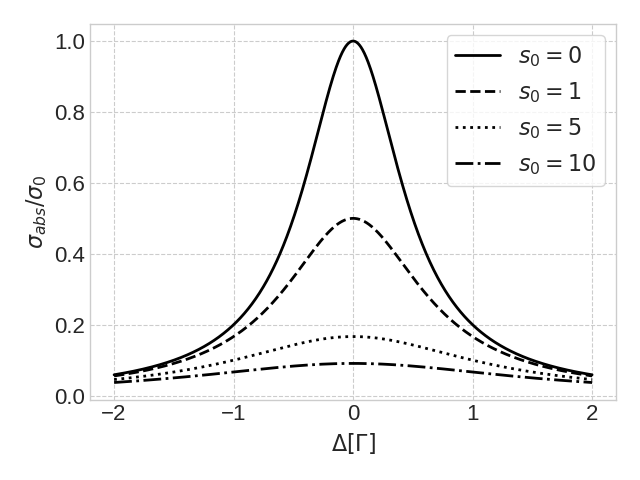
\includegraphics[width=0.5\textwidth]{USPSC-img/net_absorption_cross_section.png}
	\vspace{-5pt}
	\legend{Net absorption cross section as function of detuning for some values of resonant saturation parameter.\\ Source: Author}
	\label{fig:net-absorption-cross-section}
\end{figure}

%-----------------------------------
\subsection{Doppler broadening}
\label{sec:Doppler-broadening}
%-----------------------------------

The angular frequency $ \omega' $ of an incident light beam depends on the frame in which it is being observed. This effect is known as \textbf{Doppler effect}. We have been studying the atom-light interaction assuming that the light frequency is the same in both laboratory and atom frames. However, the Doppler effect causes an \textit{inhomogeneous resonance shift} since each atom will perceive an angular frequency given by
\begin{equation}
	\omega' = \omega - \mathbf{k} \cdot \mathbf{v},
	\label{eq:Doppler-effect}
\end{equation}
where $ \omega $ and $ \mathbf{k} $ are, respectively, the angular frequency and the wave vector of the light beam in the laboratory frame, and $ \mathbf{v} $ is the velocity of the atom also in the laboratory frame. Subtracting the resonant angular frequency $ \omega_0 $ in both sides of equation (\ref{eq:Doppler-effect}), we obtain
\begin{equation}
	\Delta_{eff} = \Delta - \mathbf{k} \cdot \mathbf{v},
	\label{eq:Doppler-shift}
\end{equation}
where $ \Delta_{eff} = \omega' - \omega_0 $ is the \textit{effective detuning}. We must called $ -\mathbf{k} \cdot \mathbf{v} $ as \textbf{Doppler shift}. Let us consider a gas following the \textit{Maxwell-Boltzmann distribution} so that the probability $ P(v) dv $ of finding an atom with a velocity component between $ v $ and $ v + dv $ parallel to $ \mathbf{k} $ direction is given by
\begin{equation}
	P(v) dv = \frac{1}{\alpha\sqrt{2\pi}} \exp\left(-\frac{v^2}{2\alpha^2}\right) dv,\ \ \alpha \equiv \sqrt{\frac{k_B T}{m}},
	\label{eq:Maxwell-Boltzmann-distribution}
\end{equation}
where $ T $ is the temperature of the gas, $ k_B $ is the Boltzmann constant, and $ m $ is the atom mass. The equation (\ref{eq:Maxwell-Boltzmann-distribution}) is a \textbf{Gaussian distribution} centered at zero whose \textit{standard deviation} is $ \alpha $. Also, the FWHM is approximately $ 2.355 \alpha $. If we consider a resonant laser so that $ \Delta = 0 $ or $ \omega = \omega_0 $, we can associated an effective absorption line shape given by
\begin{equation}
	D(\omega') = \frac{1}{\beta \sqrt{2\pi}} \exp\left[-\frac{(\omega' - \omega_0)^2}{2\beta^2}\right],\ \ \beta \equiv \frac{\omega_0}{c} \alpha = \frac{\omega_0}{c} \sqrt{\frac{k_b T}{m}}.
\end{equation}
%-----------------------------------
%

% Optical Forces
%-----------------------------------
%\input{USPSC-TA-Textual/Atom-Light-Interaction/Forces-Two-Level-Atoms.tex}
%-----------------------------------
%

% Considerations about multi-level atoms
%-----------------------------------
%\input{USPSC-TA-Textual/Atom-Light-Interaction/Multi-level-atoms.tex}
%-----------------------------------
%


	% ---
	% Magneto-Optical Trap
	% ---
	%
%--- 
%-----------------------------------
\chapter{Magneto-Optical Trap}
\label{ch:MOT}
%-----------------------------------
%--- 
%

The magneto-optical trap (MOT) is a technique widely used in laser cooling experiments which allows both trapping and cooling of an atomic dilute gas. In this section, we shall approach the MOT theory \cite{krzysztof2010magneto, perrin2014doppler} considering the simplest transition $ J = 0 \rightarrow J = 1$, where $ J $ is the total angular momentum of the electronic state. To get an insight into the cooling and trapping mechanisms, we introduce a simplified one-dimensional MOT (1D-MOT) assuming two counter-propagating laser beams and a linear magnetic field\footnote{A linear magnetic field is not a real magnetic field since it does not satisfy the Gauss's law for magnetism.}. The three-dimensional case is more complicated to approach since there are considerable difficulties related to the complex spatial structure of the light field \cite{prudnikov2015three}, which hampers a quantitative analysis. We briefly discuss this case such nuances. Lastly, we introduce \textbf{narrow-line magneto-optical traps} (nMOTs) \cite{loftus2004narrow} by assuming an atomic transition with a natural linewidth (section \ref{sec:line-broadening-mechanisms}) close to the photonic recoil.

% One-dimensinal case
%-----------------------------------
%
%-----------------------------------
\section{One-dimensional model}
\label{sec:one-dimensional-model}
%-----------------------------------
%

Let us consider a simplified one-dimensional model (1D-MOT) illustrated in figure \ref{fig:1D-MOT}. In this model, two counter-propagating laser beams of opposite circular polarization interact with an atom in the presence of a linear magnetic field $ \mathbf{B} = B_0 z \mathbf{e}_z $, where $ B_0 > 0 $ is the gradient magnitude. Both laser beams have the same angular frequency $ \omega $ and are tuned close to the transition $ J = 0 \rightarrow J = 1 $ whose angular frequency is $ \omega_0 $.

\begin{figure}[!ht]
	\centering
	\caption{1D-MOT}
	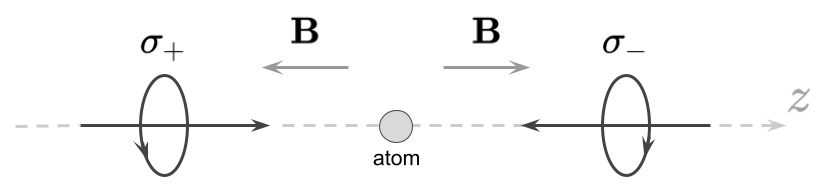
\includegraphics[width=0.7\textwidth]{USPSC-img/1D-MOT.png}
	\vspace{5pt}
	\legend{Simplified one-dimensional MOT composed of two counter-propagating laser beams and a linear magnetic field $ \mathbf{B} = B_0 z \mathbf{e}_z $, where $ B_0 > 0 $. We consider the $ \sigma_{+} $ and $ \sigma_{-} $ beams right-handed and left-handed polarized respectively. \\ Source: Author}
	\label{fig:1D-MOT}
	\vspace{-10pt}
\end{figure}

Disregarding the magnetic field, the transition is properly represented by a degenerate \textit{two-level system} whose energy difference is $ \hbar \omega_0 $. The presence of the magnetic field splits the energy level $ J = 1 $ into three different energy levels $ m_J = 0, \pm 1 $ such that the system turns into a \textit{four-level system} illustrated in figure \ref{fig:1D-MOT-Zeeman-splitting}. This effect is known as \textbf{Zeeman splitting} \cite[Section~7.4]{steck2007quantum}. Essentially, assuming a weak magnetic field\footnote{The quantity $ \mu_B B $, where $ B $ is the magnetic field magnitude, must be much lower than the spin-orbit coupling energy.}, there will be a effective detuning $ \delta_Z^{(m_J)} $ due to the \textbf{anomalous Zeeman effect} so that
\begin{equation}
	\delta_Z^{(m_J)} = - \beta g_{J} m_J z,\ \ \textrm{being}\ \ \beta \equiv \frac{\mu_B B_0}{\hbar},
	\label{eq:Zeeman-shift}
\end{equation}
where $ g_J $ is the \textit{Landé factor} and $ \mu_B $ is the Bohr magneton. The equation (\ref{eq:Zeeman-shift}) is also called \textbf{Zeeman shift}. It is relevant to notice that the detuning depends linearly on the position $ z $ so that $ \delta_Z^{(m_J)} \propto z $.

\begin{figure}[!ht]
	\centering
	\caption{Zeeman splitting in 1D-MOTs}
	\includegraphics[width=0.7\textwidth]{USPSC-img/1D-MOT-Zeeman-splitting.png}
	\vspace{5pt}
	\legend{Zeeman splitting of the transition $ J = 0 \rightarrow J = 1 $ in 1D-MOTs. When $ \mathbf{B} = 0 $ ($\mathbf{B}$ off), the atomic transition $ J = 0 \rightarrow J = 1 $ is described by a \textbf{degenerate two-level system}. However, when $ \mathbf{B} \neq 0 $ ($\mathbf{B}$ on), the same atomic transition is represented by a \textbf{four-level system} in which the excited states are energetically separeted by the Zeeman shift $ \delta_{Z}^{(\pm)} $. The energy scale was not plotted precisely to enhance the visibility.\\ Source: Author}
	\label{fig:1D-MOT-Zeeman-splitting}
\end{figure}

%-----------------------------------
\subsection{Cooling and trapping effect}
\label{sec:cooling-trapping-effect}
%-----------------------------------

Let us consider an arbitrary atom from an atomic cloud in a MOT neglecting interatomic interactions. Although the momentum exchange between atoms and light are quantized, we can evaluate the atom dynamics classically by assuming a mean force $ \mathbf{F}_{MOT} $, which is known as \textbf{semiclassical approach}. It is possible to obtain an analytical expression for $ \mathbf{F}_{MOT} $ under the \textbf{two-level system approximation}, which will be done in the next section \ref{sec:MOT-force}. Without this approximation, we must consider the interplay between optical pumping, photon scattering, Zeeman effect, and Doppler effect in multiple excited states. Therefore, the complexity of the problem will increase considerably. There are only a few articles \cite{prudnikov2015three, choi2008three, PhysRevA.49.4864} that approach this case.

We can be split $ \mathbf{F}_{MOT} $ into two components\footnote{In section \ref{sec:optical-forces}, we deduced both forces for the case of a two-level atom interacting with a single field.}: one exclusively associated with coherent transitions (absorption and \textit{stimulated} emission); and another associated with decoherence decays (absorption and \textit{spontaneous} emission). In weak atom-light coupling, stimulated emission is much less often than spontaneous emission. Therefore, $ \mathbf{F}_{MOT} $ is the \textbf{radiation pressure force}. Essentially, $ \mathbf{F}_{MOT} = (F_{+} - F_{-}) \mathbf{e}_z $, where $ F_{\pm} $ is related to the interaction between atom and the $ \sigma_{\pm} $-beam. Thus, $ F_{\pm} $ depends on the detuning $ \Delta_{\pm} $ so that the lower $ |\Delta_{\pm}| $, the greater $ F_{\pm} $. The detuning $ \Delta_{\pm} $ can be split into three detunings (figure \ref{fig:detuning-1D-MOT}) so that $ \Delta_{\pm} = \delta + \delta_Z^{\pm} + \delta_D^{\pm} $. These detunings are given by
\begin{itemize}
	\item \textit{Laser detuning} $ \delta = \omega - \omega_0 $: associated with the laser frequency $ \omega $ and the energy difference $ \omega_0 $ of the atomic transition. This detuning is the same for all transitions;

	\item \textit{Doppler shift} $ \delta_{D}^{(\pm)} = \mp k v $: associated with the atomic movement (see section \ref{sec:line-broadening-mechanisms});

	\item \textit{Zeeman shift} $ \delta_Z^{(\pm)} \propto \mp z $: associated with the Zeeman splitting. This detuning is given by the equation (\ref{eq:Zeeman-shift}).
\end{itemize}

\begin{figure}[!ht]
	\centering
	\caption{Detuning in 1D-MOT}
	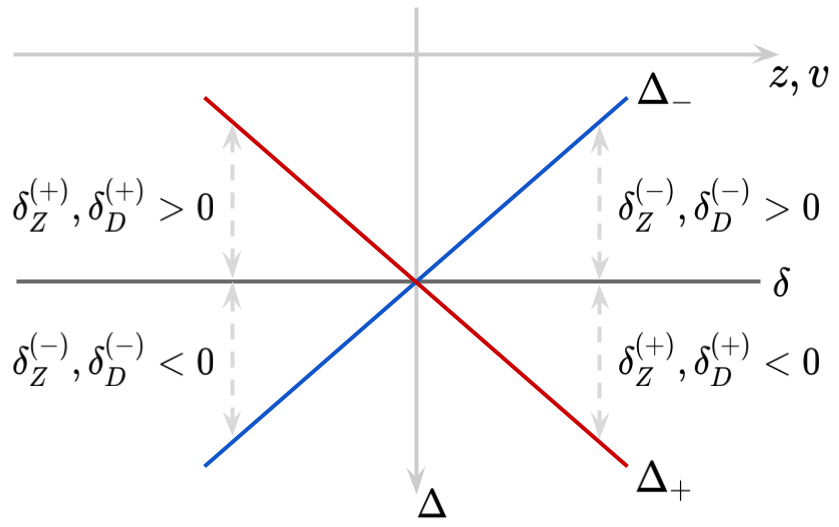
\includegraphics[width=0.55\textwidth]{USPSC-img/1D-MOT-detunings.png}
	\vspace{5pt}
	\legend{Laser detuning, Doppler shift, and Zeeman shift of a 1D-MOT in function of velocity $ v $ and position $ z $ assuming red-detuned laser beams ($ \delta < 0 $). \\ Source: Author}
	\label{fig:detuning-1D-MOT}
	\vspace{-20pt}
\end{figure}

Both Doppler shift and Zeeman shift increase linearly with the atom velocity and atom position respectively. Assuming red-detuned laser beams ($ \delta < 0 $) and $ v > 0 $, the probability of absorbing the $ \sigma_{\pm} $-beam decreases (increase) with $ v $ since $ |\Delta_{\pm}| $ increases (decreases). When $ v < 0 $, the opposite effect occurs. Therefore, the MOT force is opposite to the velocity $ v $ ($ \partial \mathbf{F}_{MOT} / \partial v < 0 $) such as a friction, which is is essentially a \textbf{cooling mechanism} also known as \textbf{Doppler cooling}. The Zeeman shift behaves the same in function of $ z $ such that the MOT force is also opposite to the position ($ \partial \mathbf{F}_{MOT} / \partial z < 0 $), which is essentially a \textbf{trapping mechanism}.

%-----------------------------------
\subsection{MOT Force}
\label{sec:MOT-force}
%-----------------------------------

We shall get deeper into the 1D-MOT analysis by quantifying the MOT force. As mentioned in section \ref{sec:cooling-trapping-effect}, obtain an analytical expression for the MOT forces in the general case is a complicated task. Although, we can obtain such analytical expression under two approximations:
\begin{itemize}
	\item By breaking the four-level system (figure \ref{fig:1D-MOT-Zeeman-splitting}) into three independent two-level systems illustrated in figure \ref{fig:independent-two-level-system}. That is a strong assumption in which the coherence effects between the Zeeman states, such as Raman-like transitions \cite[Section~9.8]{foot2005atomic}, are neglected;

	\item By assuming that the atom density operator $ \hat{\rho}(\mathbf{k}, -\mathbf{k}) $ related to the simultaneous interaction equals the sum of the density operators $ \hat{\rho}_{+}(\mathbf{k}) $ and $ \hat{\rho}_{-}(-\mathbf{k}) $ associated with the individual interactions, which is essentially a superposition ($ \hat{\rho} = \hat{\rho}_{+} + \hat{\rho}_{-} $). This approximation relies on the perturbation theory in first and second-order \cite[Chapter~7]{berman2011principles}. 
\end{itemize}

Both approximations are valid in the regime of weak atom-light coupling so that the total detuning is higher than the power-broadened linewidth.

\begin{figure}[!ht]
	\centering
	\caption{Assumption of independent two-level systems}
	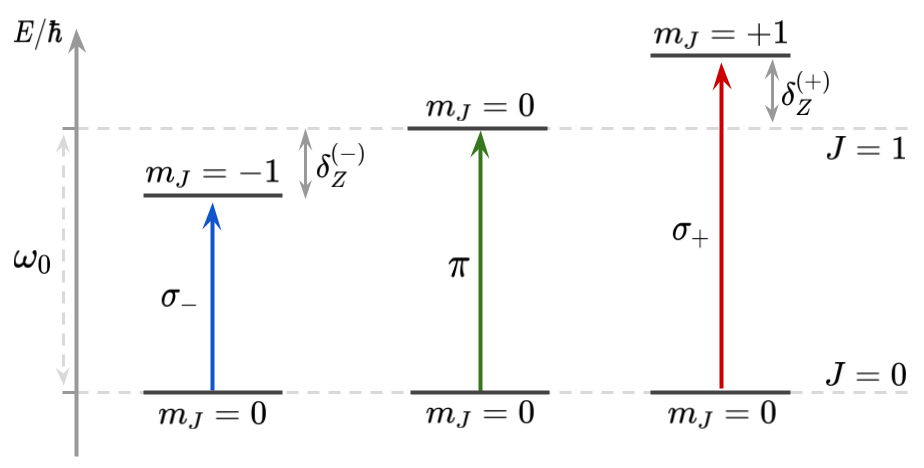
\includegraphics[width=0.6\textwidth]{USPSC-img/Independent-two-level-system.png}
	\legend{Breaking of the four-level system into three independent two-level systems.\\ Source: Author}
	\label{fig:independent-two-level-system}
\end{figure}

Since there are only right-handed and left-handed polarized beams, there will only $ \sigma_{\pm} $-transitions. Therefore, the components $ F_{+} $ and $ F_{-} $ associated with the $ \sigma_{+} $ and $ \sigma_{-} $ transitions respectively are independent radiation pressure forces given by (see section \ref{sec:optical-forces})
\begin{equation}
	F_{\pm}(z, v) = \pm \hbar k \frac{\Gamma}{2} \frac{s_0}{1 + s_0 + 4(\Delta_{\pm} / \Gamma)^2},
	\label{eq:1D-MOT-force-components}
\end{equation}
where $ \Delta_{\pm} = \delta + \delta_{Z}^{(\pm)} + \delta_{D}^{(\pm)} $, $ s_0 $ is the saturation parameter, and $ \Gamma $ is the natural linewidth\footnote{The natural linewidth depends on the energy difference between the states, which is slightly different in each transition. However, this energy difference is much lower than $ \hbar \omega_0 $ such that the natural linewidth is approximately $ \Gamma $.} of the transition $ J = 0 \rightarrow J = 1 $. Assuming low velocities ($ |kv| \ll |\delta| $) and positions close to the magnetic field centre ($ |z| \ll |\delta| $), the MOT force is essentially linear with $ z $ and $ v $ as illustrated in figure \ref{fig:MOT-force}. Hence, we can expand $ F_{MOT} $ about $ z = 0 $ and $ v = 0 $ so that
\begin{equation}
	F_{MOT}(z, v) \simeq F_{MOT}(0, 0) + z \frac{\partial F_{MOT}}{\partial z}(0, 0) + v \frac{\partial F_{MOT}}{\partial v}(0, 0),
	\label{eq:MOT-force-Taylor-expansion}
\end{equation}

\begin{figure}[!ht]
	\centering
	\caption{MOT force}
	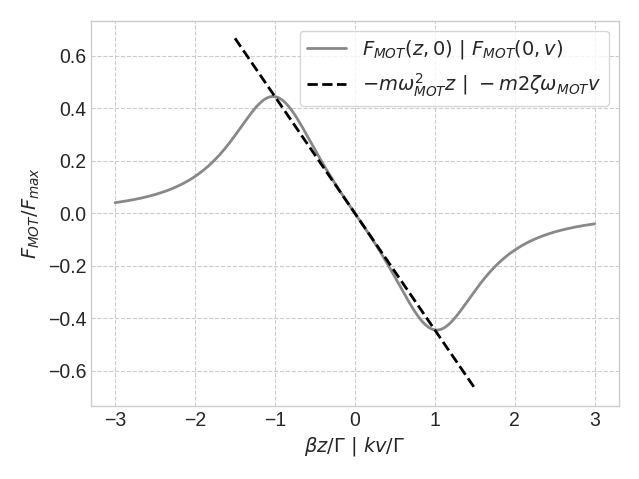
\includegraphics[width=0.5\textwidth]{USPSC-img/MOT_force.png}
	\legend{Plotting of the MOT force $ F_{MOT} $ for $ v = 0 $ ($ z = 0 $) in function of $ \beta z / \Gamma $ ($ k v / \Gamma $) considering the transition $ {}^{1}S_0 \rightarrow {}^{1}P_1 $ of the $ {}^{88}Sr $ for $ \delta = - \Gamma $ and $ s_0 = 1 $. The dashed line in the graph is the MOT force assuming $ |\beta z| \ll |\delta| $ ($ |kv| \ll |\delta| $).\\ Source: Author}
	\label{fig:MOT-force}
\end{figure}

Rearranging the terms of equation (\ref{eq:MOT-force-Taylor-expansion}), we obtain
\begin{gather}
	\frac{d^2 z}{dt^2} + 2\zeta \omega_{MOT} \frac{d z}{d t} + \omega_{MOT}^2 z = 0,
	\label{eq:damped-harmonic-oscillation-1D-MOT}
	\\
	\omega_{MOT}^2 \equiv - \frac{1}{m} \frac{8 \hbar k \beta g_J s_0 (\delta / \Gamma)}{[1 + s_0 + 4(\delta / \Gamma)^2]^2},\ \ \textrm{and}\ \ \zeta \equiv \frac{k}{2\beta g_J} \omega_{MOT},
	\label{eq:constants-equation-of-motion-1D-MOT}
\end{gather}
where $ m $ is the atomic mass. The quantity $ \omega_{MOT} $ has unit of frequency and $ \zeta $ is a dimensionless quantity. Also, $ \omega_{MOT}^2 $ is a positive real value since we are assuming red-detuned lasers, which means $ \delta < 0 $ in equation \ref{eq:constants-equation-of-motion-1D-MOT}. The equation of motion (\ref{eq:damped-harmonic-oscillation-1D-MOT}) describes a \textit{damped harmonic oscillation} of which $ \omega_{MOT} $ is the \textit{undamped frequency} and $ \zeta $ is the \textit{damping ratio}. Therefore, the atom is trapped by the restoring force $ - m \omega_{MOT}^2 z $, being limited to move in a restricted region (\textbf{trapping mechanism}). Furthermore, the atom loses energy due to the damping $ 2 \zeta \omega_{MOT} v $ can be understood as a \textbf{cooling mechanism}.

%-----------------------------------
%

% Three-dimensional case
%-----------------------------------
%
%-----------------------------------
\section{Three-dimensional case}
\label{eq:three-dimensional-case}
%-----------------------------------
%
\begin{wrapfigure}{l}{0.5\textwidth}
	\centering
	\caption{Standard 3D-MOT arrangement}
	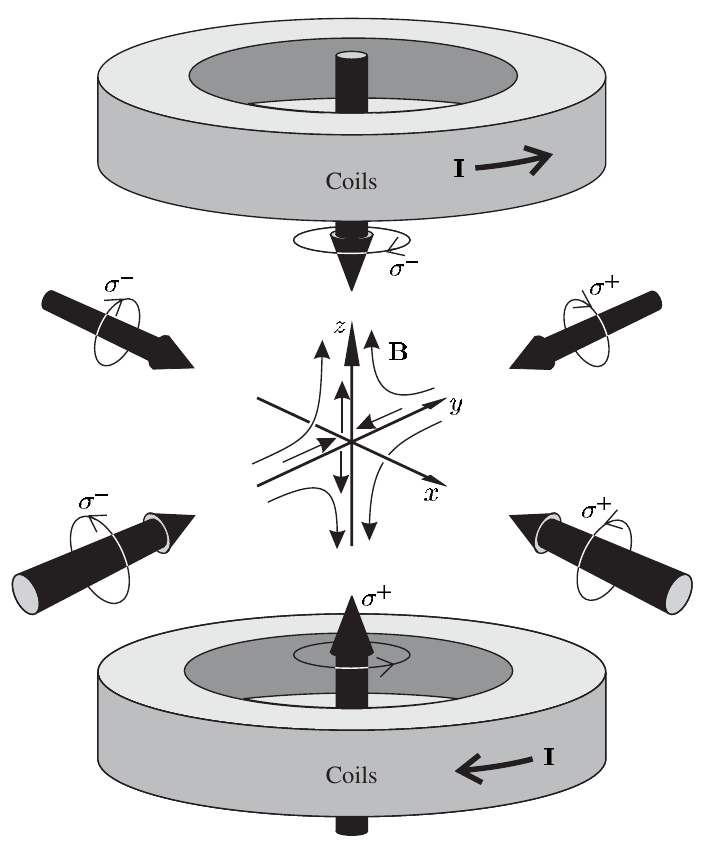
\includegraphics[width=0.45\textwidth]{USPSC-img/standard-3D-MOT-arrangement.png}
	\legend{Standard arrangement of MOT composed of three orthogonal pairs of counter propagating laser beams with opposite circular polarization and coils in anti-Helmholtz configuration, which produces a magnetic quadrupole field. \\ Source: \cite[Figure~9.9]{foot2005atomic}}
	\label{fig:standard-3D-MOT-arrangement}
	\vspace{-20pt}
\end{wrapfigure}
Let us assume the standard 3D-MOT arrangement illustrated in figure \ref{fig:standard-3D-MOT-arrangement}. An atom, free to move along all Cartesian axes, interacts with \textit{three pairs} of counter-propagating laser beams with opposite circular polarization and a magnetic quadrupole field $ \mathbf{B} $. In a first attempt, we can naturally extend the 1D-MOT theory into a 3D theory considering that each laser beam yields a radiation pressure force given by equation (\ref{eq:1D-MOT-force-components}). Nevertheless, the quantization axis ($z$-axis) must match the direction of the field $ \mathbf{B} $ to proper evaluate the Zeeman shift, which implies that each laser beam polarization depends on the atomic position. This is not a concern in the 1D-MOT since the magnetic field has a fixed direction. Therefore, a theoretical description of the 3D-MOT \cite{prudnikov2015three} encounters considerable difficult due to the spatial-dependence of the quantization axis. Regardless the theoretical complications, the cooling and trapping effects of MOTs are widely confirmed for many alkali \cite{raab1987trapping, katori1999magneto, zachorowski1998magneto} and lanthanide \cite{maier2014narrow, miyazawa2021narrow, frisch2012narrow}. Also, in this thesis, we could demonstrate both effects for dysprosium and strontium atoms through a stochastic simulation. Moreover, it is possible to estimate temperature and also atomic cloud size.

%-----------------------------------
\subsection{Limit temperature in Doppler cooling}
\label{sec:Doppler-temperature-limit}
%-----------------------------------

Let us consider a equilibrium atomic position close to the magnetic field centre. In this case, the Zeeman shift becomes negligible compared to the Doppler shift ($ \delta_{Z} \ll \delta_{D} $) such that a defined quantization axis is no longer required. \footnote{Essentially, we are proposing the treatment of a MOT as an \textbf{optical molasses}, which is a similar technique to only cool an atomic dilute gas based upon \textit{Doppler cooling}.} Also, we suppose weak atom-light couplings in which the laser detuning are grater than the power-broadened linewidth. Thus, the interaction between each laser beam and the atom is independent and it is described by two-level dynamics. In this situation, the MOT force is given by
\begin{equation}
	\mathbf{F}_{MOT}(\mathbf{v}) = \frac{\hbar k \Gamma s_0}{2} \sum_{n = 1}^{3} \left( \frac{1}{1 + s_0 + 4[\delta - k (\mathbf{v} \cdot \mathbf{e}_n)]^2 / \Gamma^2} - \frac{1}{1 + s_0 + 4[\delta + k (\mathbf{v} \cdot \mathbf{e}_n)]^2 / \Gamma^2} \right)\mathbf{e}_{n},
\end{equation}
where $ \{ \mathbf{e}_1, \mathbf{e}_2, \mathbf{e}_3 \}$ is the Cartesian basis. We are assuming all laser beams with the same saturation parameter $ s_0 $, wavevector magnitude $ k $, and detuning $ \delta $. For low velocities $ v $ such that $ kv \ll \delta $, we can expand the MOT force around $ \mathbf{v} = 0 $ so that $ \mathbf{F}_{MOT} \simeq - \gamma \mathbf{v} $,
\begin{equation}
	\gamma = - \frac{8 \hbar k^2 s_0 (\delta / \Gamma)}{[1 + s_0 + 4(\delta / \Gamma)^2]^2}.
\end{equation}
Assuming red-detuned laser beams ($ \delta < 0 $), we have $ \gamma > 0 $ and then $ \mathbf{F}_{MOT} $ describes a friction force. Hence, the velocity vanishes after a time as long as $ 1 / \gamma $ and then the final temperature should be zero. However, the $ \mathbf{F}_{MOT} $ is an average and therefore we must take its fluctuations into account. These fluctuations are associate with the Brownian atomic motion due to spontaneous emission, which yields a \textit{heating process}. Therefore, a finite temperature is set by the balance between cooling and heating mechanisms. 

Let us considering a cycle of $ N $ 

%-----------------------------------
\subsection{Atomic cloud size}
\label{sec:MOT-cloud-size}
%-----------------------------------
%-----------------------------------
%

% Narrow Line Magneto-Optical Trap
%-----------------------------------
%
%-----------------------------------
\newpage
\section{Narrow-line magneto-optical trap}
%-----------------------------------
%

\begin{wrapfigure}{l}{0.4\textwidth}
    \centering
    \vspace{-10px}
    \caption{Atomic cloud shape in nMOTs for small laser intensities.}
    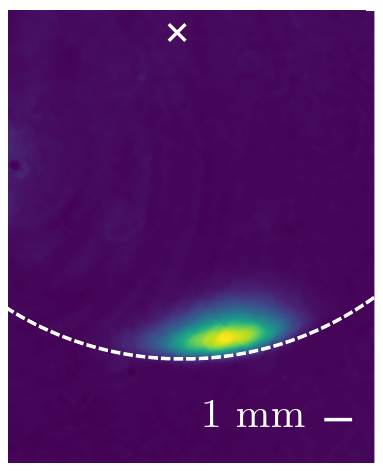
\includegraphics[width=0.3\textwidth]{USPSC-img/atomic_cloud_shape_in_nMOTs.png}
    \legend{Typical \textit{in situ} absorption image of an atomic sample in a nMOT. \\ Source: \cite{dreon2017optical}}
    \label{fig:atomic-cloud-shape-nMOTs}
    \vspace{-10px}
\end{wrapfigure}

In previous sections, we have been neglecting the gravity effect on the MOT parameters. This assumption is valid when the MOT force is much higher than gravity. The maximum radiation pressure force on an atom is $ \hbar k \Gamma / 2 $ from equation (\ref{eq:1D-MOT-force-components}). Therefore, the ratio between the maximum radiation pressure force and gravity is
\begin{equation}
    R \equiv \frac{\hbar k \Gamma}{2 m g},
    \label{eq:gravity-radiation-force-ratio}
\end{equation}
where $ m $ is the atomic mass and $ g $ is the gravitation acceleration. Usually, $ R $ is on the order of $ 10^5 $. Hence, the gravity force is negligible since the radiation pressure force is much higher. However, the lower $ \Gamma $, the higher the gravity effect so that for $ \Gamma \sim\ \textrm{kHz} $, the ratio (\ref{eq:gravity-radiation-force-ratio}) approaches values on the order of $ 10 $. In this case, the centre of mass moves towards the gravity direction such that, for small laser intensities, the atoms gather on the bottom of the surface of an ellipsoid as illustrated in figure \ref{fig:atomic-cloud-shape-nMOTs}.

Furthermore, $ \Gamma $ also defines the average number of scattering events per time (\textbf{scattering rate}) so that the lower $ \Gamma $, the fewer the number of events in a determined time interval. We have been analysing the atoms dynamics classically through the optical forces, which assumes that there are a large number of momentum exchange in a small period of time. In this condition, we can average out a force. That is not satisfied when $ \Gamma $ is sufficient smaller. In this case, we must include the discrete momentum exchange in the analysis and then treat the dynamics quantum mechanically. To quantify the range of $ \Gamma $ in which this happens, let us define the ratio given by
\begin{equation}
    \eta = \frac{\Gamma}{\omega_R} = \frac{m \lambda^2 \Gamma}{2\pi^2 \hbar} =
    \label{eq:narrowness}
\end{equation}
where $ \hbar \omega_R $ is the kinetic energy $ (\hbar k)^2 / (2 m) $ gain by the atom when it absorbs an photon with the momentum $ \hbar k $, $ h $ is the Planck constant, and $ \lambda = 2\pi/k $ is the wavelength. This energy is known as \textbf{photonic recoil}. When $ \eta \leq 1 $, one scattering event is able to detune the atom-light interaction. A MOT whose $ \eta \sim 1 $ or less is known as \textbf{narrow-line magneto-optical trap} (nMOT), whereas a MOT whose $ \eta \gg 1 $ is known as \textbf{broad-line magneto-optical trap}. We shall call the ratio (\ref{eq:narrowness}) as \textbf{narrowness}.


%-----------------------------------
\subsection{Operating regimes}
\label{sec:nMOT-operating-regimes}
%-----------------------------------

Four quantities play a crucial role in nMOTs operating: the saturation parameter $ s_0 $, the laser detuning $ \delta $, the natural linewidth $ \Gamma $, and the photonic recoil $ \omega_R $. We can combined $ s_0 $ and $ \Gamma $ in a single quantity known as \textbf{power-broadened linewidth} $ \Gamma' \equiv \Gamma \sqrt{1 + s_0} $, which is the natural energy scale of the atom-light interaction due to the power-broadening mechanism (section \ref{sec:line-broadening-mechanisms}). Furthermore, we can summarize those quantities in two essential quantities that characterized nMOTs:
\begin{itemize}
    \item ($ \eta' \equiv \Gamma' / \omega_R $): it defines the relevance of single scattering events to the the atom-light interaction taking the natural energy scale into account. Hence, $ \eta' $ is more accurate than $ \eta $;
    \item ($ \delta' \equiv \delta / \Gamma' $): it defines the coupling strength between atom and light normalized by the natural energy scale of the interaction.
\end{itemize}
When $ \eta' \gg 1 $, the semiclassical approach is suitable since the photonic recoil is much lower than the natural energy scale and, therefore, the scattering events can be averaged out. There are three nMOTs regimes:
\begin{enumerate}
    \item[I] \textbf{Doppler regime} ($ \eta' \gg 1 $ and $ |\delta'| < 1 $): in this regime, gravity is negligible so that the atomic cloud is ellipsoidal;
    \item[II] \textbf{Power-broadened regime} ($ \eta' \gg 1 $ and $ |\delta'| > 1 $): In this regime, gravity is comparable to the radiation pressure forces such that the atomic cloud centre of mass sags to vertical positions.
    \item[III] \textbf{Quantum regime} ($ \eta' \sim 1 $): in this regime, the photonic recoil is the natural energy scale and, therefore, the quantum physics governs the nMOT dynamics.
\end{enumerate}

%-----------------------------------
\subsection{Centre of mass of the atomic cloud}
\label{sec:nMOT-centre-of-mass}
%-----------------------------------

We can estimate the centre of mass of the atomic cloud in the power-broadened regime by assuming that all radiation pressure forces on an atom balance each other in all directions except in the gravity direction $ \hat{z} $. In this direction, the radiation pressure forces $ F_{\pm} $ balance with the gravity force as illustrated in figure \ref{fig:forces-diagram-trapped-atom-nMOT-power-broadened-regime}.
\begin{figure}[!ht]
    \centering
    \caption{Forces diagram of a trapped atom}
    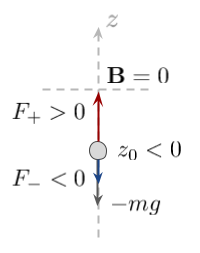
\includegraphics[width=0.17\textwidth]{USPSC-img/centre_of_mass_power_broadened_regime.png}
    \legend{Forces diagram of a trapped atom in a power-broadened nMOT. \\ Source: author}
    \label{fig:forces-diagram-trapped-atom-nMOT-power-broadened-regime}
    \vspace{-10px}
\end{figure}
Thus, a trapped atom is restricted to be in a region where the magnetic field components perpendicular to $ z $ is zero, otherwise there will be unbalance between forces in those direction due to the Zeeman shift (see section \ref{sec:cooling-trapping-effect}). The average position of a trapped atom must be $ \vec{r} = z_0 \hat{z} $ so that its dynamics is well described by the one-dimensional model presented in section \ref{sec:one-dimensional-model}. From equations (\ref{eq:1D-MOT-force-components}), we obtain the following equation of motion
\begin{equation}
    \hbar k \frac{\Gamma}{2} s_0 \left( \frac{1}{1 + s_0 + 4(\Delta_{+} / \Gamma)^2} - \frac{1}{1 + s_0 + 4(\Delta_{-} / \Gamma)^2}  \right) - mg = 0.
    \label{eq:equation-motion-1D-model-under-gravity}
\end{equation}
We must impose $ |\Delta_{+}| < |\Delta_{-}| $ to ensure a solution to the equation (\ref{eq:equation-motion-1D-model-under-gravity}). Neglecting the Doppler shift ($ \delta_{D}^{(\pm)} = 0 $), and assuming red-detuned lasers\footnote{This assumption is necessary to create a trapping environment as discussed in \ref{sec:cooling-trapping-effect}.} ($ \delta < 0 $), we obtain $ z_0 < 0 $, which means the centre of mass will be located below the magnetic field origin. Let us consider $ |\delta| \gg 1 $ so that $ |\Delta_{+}| \gg |\Delta_{-}| $. In this condition, $ F_{-} $ is negligible. Hence, we can approximate the equation (\ref{eq:equation-motion-1D-model-under-gravity}) to
\begin{equation}
    \hbar k \frac{\Gamma}{2} s_0 \left( \frac{1}{1 + s_0 + 4[(\delta + \delta_{Z}^{(+)}) / \Gamma]^2}\right) - mg = 0.
\end{equation}
We have been assuming the transition $ J = 0 \longrightarrow J = 1 $ such that $ \delta_Z^{(+)} = - \beta g_J m_J z $. However, the transition can happen between any transition $ J = j \longrightarrow J = j + 1$, where $ j \geq 0 $. To take it into account, we must consider
\begin{equation}
     \delta_Z^{(+)} = - \beta \chi z_0,\ \textrm{being}\ \chi \equiv (g_J - g_J') j > 0,
     \label{eq:zeeman-shift-generic-transition}
\end{equation}
where $ g_J' $ and $ g_J $ are the \textit{Landé factors} of the excited and ground states respectively. The equation (\ref{eq:zeeman-shift-generic-transition}) is valid when the transitions only happens between the states $ m_J = -j $ and $ m_J = -j + 1 $. Isolating $ z_0 $, we obtain
\begin{equation}
    z_0 = - \frac{1}{\beta \chi} \left(\delta + \frac{\Gamma}{2} \sqrt{\frac{h \Gamma s_0}{2 \lambda m g} - 1 - s_0} \right)
    \label{eq:centre-of-mass-power-broadened-regime}
\end{equation}
The equation (\ref{eq:centre-of-mass-power-broadened-regime}) is only valid when the centre of mass is sufficient below the magnetic field origin to match all the assumptions described above and in section \ref{sec:MOT-force}.

%-----------------------------------
%


	% ---
	% nMOT Stochastic Dynamics
	% ---
	%
%--- 
%-----------------------------------
\chapter{nMOT stochastic dynamics}
\label{ch:simulation}
%-----------------------------------
%--- 
%

% Markovian evolution
%-----------------------------------
\input{USPSC-TA-Textual/Stochastic-dynamics/Markovian-evolution.tex}
%-----------------------------------
%

% Monte Carlo Simulation
%-----------------------------------
%
%-----------------------------------
\section{Monte Carlo simulation}
\label{sec:monte-carlo-simulation}
%-----------------------------------
%

%-----------------------------------
%

% Data Processing
%-----------------------------------
%
%-----------------------------------
\section{Data processing}
\label{sec:data-processing}
%-----------------------------------
%

%-----------------------------------
%

	% ---
	% Results
	% ---
	%
%--- 
%-----------------------------------
\chapter{Results}
\label{ch:results}
%-----------------------------------
%---
% 

To validate out model, we apply it to three nMOTs arrangements from different laboratories. One of them traps dysprosium atoms, whereas the others two trap strontium atoms.

% Dysprosium
%-----------------------------------
%
%-----------------------------------
\section{Dysprosium nMOT}
\label{sec:dysprosium-nMOT}
%-----------------------------------
%

We choose to simulate the dysprosium nMOT \cite{dreon2017optical} reproduced by Davide Dreon and his research group since it matches the conditions of our model and is thorough detailed in the Dreon PhD thesis \cite{dreon2017designing}, which is necessary to improve accuracy as discussed in section \ref{sec:input-outputs}.

\begin{wrapfigure}{l}{0.5\linewidth}
    \centering
    \caption{Electronic transitions of the dysprosium nMOT}
    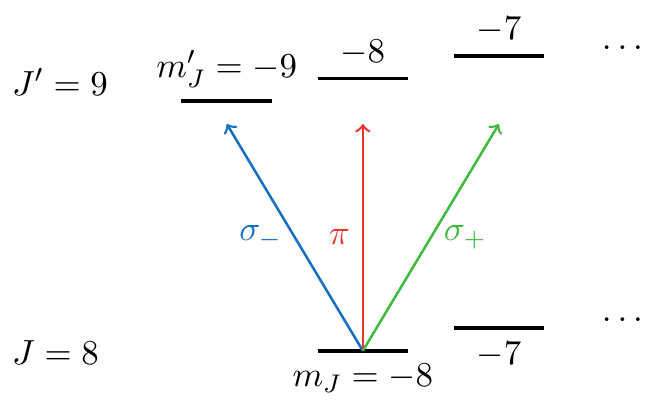
\includegraphics[width=0.45\textwidth]{USPSC-img/Dy-Dreon-transitions.png}
    \vspace{5px}
    \legend{. \\ Source: \cite{dreon2017optical}}
    \label{fig:Dy-Dreon-electronic-transitions}
\end{wrapfigure}
The involved electronic transition presented in table \ref{tab:electronic-transition-Dy-Dreon} yields a narrowness of $ \eta =  43.8 $ that is not small enough to reach the quantum regime, but it is enough to reach the power-broadened regime. Furthermore, in the presence of a magnetic field, the involved electronic transition $ J = 8 \longrightarrow J' = 9 $ has 36 possible states, which is much more complicated than the transition $ J = 0 \longrightarrow J = 1 $ presented in chapter \ref{ch:Monte-Carlo-simulation}. However, previous works \cite{lu2011strongly,aikawa2012bose} on nMOTs with Lanthanide atoms experimentally confirmed a spontaneous spin polarization that allows to simplify the transitions to $ \ket{J = 8, m_J = 8} \longrightarrow \ket{J' = 9, m_J' = -7, -8, -9} $ as  illustrated in figure \ref{fig:Dy-Dreon-electronic-transitions}.

\begin{table}[ht!]
    \centering
    \begin{tabular}{|c|c|c|}
        \hline
        \textbf{Symbol} & \textbf{Quantity} & \textbf{Value} \\ \hline
        $ \Gamma $ & Natural Linewidth & $ 2\pi \times 136\ kHz $ \\
        $ \lambda $ & Resonant wavelength & $ 626\ nm $ \\
        $ J_{gnd} $ & Ground state angular momentum & $ 8 $ \\
        $ g_{gnd} $ & Ground state Landè factor & $ 1.24 $ \\
        $ g_{exc} $ & Excited state Landè factor & $ 1.29 $ \\
        $ m $ & Mass & $ 164\ u $ \\
        \hline
    \end{tabular}
    \caption{Eletronic transition parameters of the dysprosium nMOT reproduced by \cite{dreon2017designing}.}
    \label{tab:electronic-transition-Dy-Dreon}
\end{table}

$ T_D = 3.26\ \mu K $

\begin{table}[ht!]
    \centering
    \begin{tabular}{|c|c|c|}
        \hline
        \textbf{Symbol} & \textbf{Quantity} & \textbf{Value} \\ \hline
        $ w $ & Waist & $ 2.0\ cm $ \\
        $ s_0 $ & Saturation parameter & $ 0.65 $ \\
        \hline
    \end{tabular}
    \caption{Laser setup features}
    \label{tab:lasers-setup}
\end{table}

\begin{table}[ht!]
    \centering
    \begin{tabular}{|c|c|c|}
        \hline
        \textbf{Symbol} & \textbf{Quantity} & \textbf{Value} \\ \hline
        $ B_0 $ & Axial gradient & $ 1.71 G $ \\
        $ B $ & Magnetic Field & $ B_0(-\hat{x} + \hat{y}/2 + \hat{z} / 2) $ \\
        $ B_{bias} $ & Bias & $ (-0.094 \hat{z})\ G / cm $ \\
        \hline
    \end{tabular}
    \caption{Magnetic quadrupole field}
    \label{tab:magnetic-field}
\end{table}

%-----------------------------------
\subsection{Atomic cloud profile}
\label{sec:cloud-profile-dysprosium}
%-----------------------------------

\begin{figure}[!ht]
    \centering
    \caption{Simulated ${}^{164}Dy$ cloud profile}
    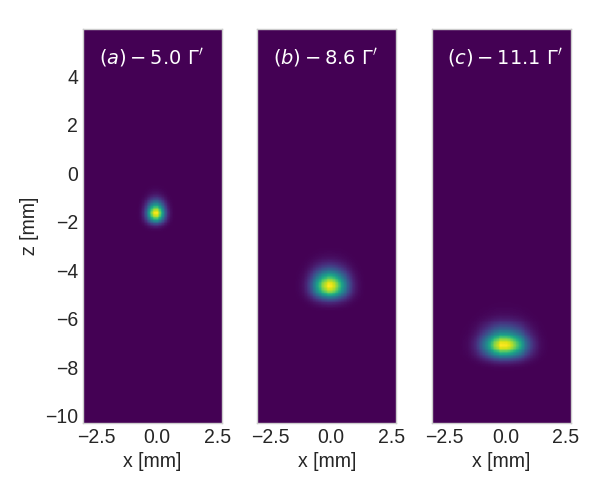
\includegraphics[width=0.7\textwidth]{USPSC-img/dy_dreon_cloud_profile.png}
    \vspace{5px}
    \legend{Simulated dysprosium cloud profile for three laser detunings: $ \delta = -5.0\Gamma' $ (a), $ \delta = -8.6\Gamma' $ (b), and $ \delta = -11.1\Gamma' $ (c), where $ \Gamma' = \Gamma \sqrt{1 + s_0} $ is the power-broadened linewidth. \\ Source: author}
    \label{fig:dy-atomic-cloud-profile}
\end{figure}

\begin{figure}[!ht]
    \centering
    \caption{Centre of mass of the ${}^{164}Dy$ nMOT}
    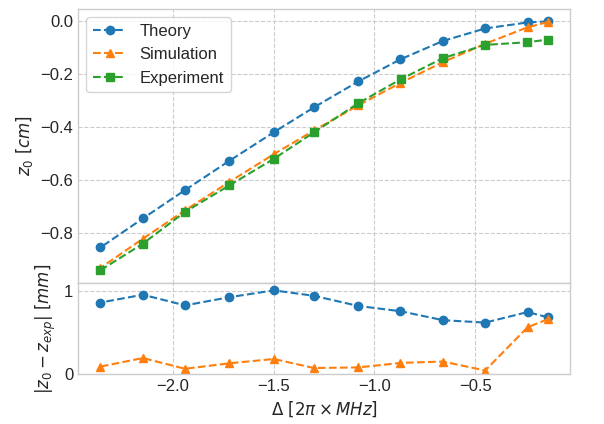
\includegraphics[width=0.7\textwidth]{USPSC-img/dy_centre_of_mass.png}
    \vspace{5px}
    \legend{centre of mass.\\ Source: author}
    \label{fig:dy-centre-of-mass}
\end{figure}

\begin{figure}[!ht]
    \centering
    \caption{Cloud size of the ${}^{164}Dy$ nMOT}
    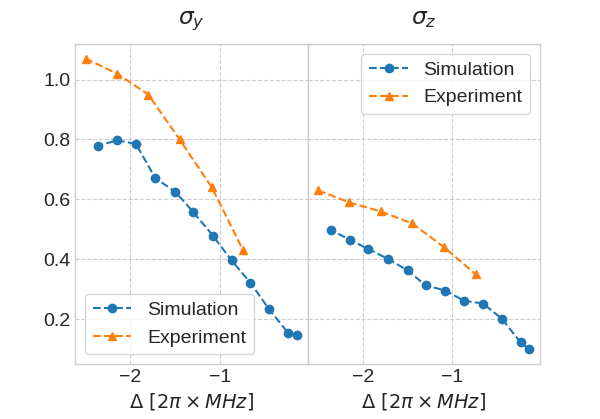
\includegraphics[width=0.7\textwidth]{USPSC-img/dy_cloud_size.png}
    \vspace{5px}
    \legend{cloud size.\\ Source: author}
    \label{fig:dy-cloud-size}
\end{figure}

\begin{figure}[!ht]
    \centering
    \caption{Cloud size ratio of the ${}^{164}Dy$ nMOT}
    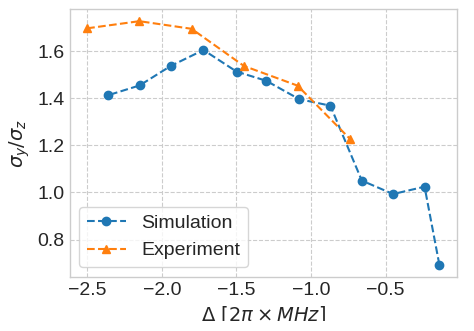
\includegraphics[width=0.55\textwidth]{USPSC-img/dy_cloud_size_ratio.png}
    \vspace{5px}
    \legend{cloud size ratio.\\ Source: author}
    \label{fig:dy-cloud-size-ratio}
\end{figure}

%-----------------------------------
\subsection{Temperature}
\label{temperature}
%-----------------------------------

\begin{figure}[!ht]
    \centering
    \caption{Temperature of the ${}^{164}Dy$ nMOT as a function of the laser detuning}
    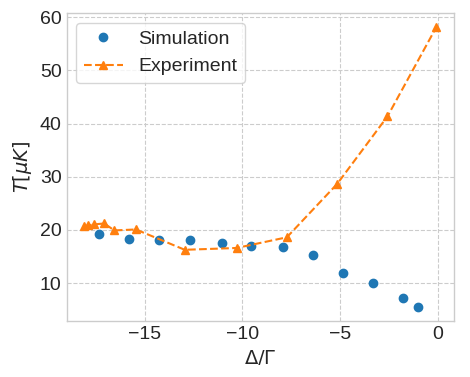
\includegraphics[width=0.6\textwidth]{USPSC-img/dy_temperature.png}
    \vspace{5px}
    \legend{temperature.\\ Source: author}
    \label{fig:dy-temperature}
\end{figure}

%-----------------------------------
%

% Strontium
%-----------------------------------
%
%-----------------------------------
\section{Strontium}
\label{eq:strontium}
%-----------------------------------
%

We shall simulate two strontium nMOTs reproduced at different laboratories. The first one, which we call \textbf{strontium-ifsc}, is managed by the research group of the professors Philippe W. Courteille at São Carlos Institute of Physics and Raul C. Teixeira at the Federal University of São Carlos. The second one, which we call \textbf{strontium-loftus}, is reported in the paper \cite{loftus2004narrow} and is one of the main references for nMOTs.

%-----------------------------------
\subsection{Atomic cloud profile}
\label{sec:cloud-profile-dysprosium}
%-----------------------------------

Experimental data from the \textit{strontium-loftus}.

\begin{figure}[!ht]
    \centering
    \caption{Simulated ${}^{88}Sr$ cloud profile}
    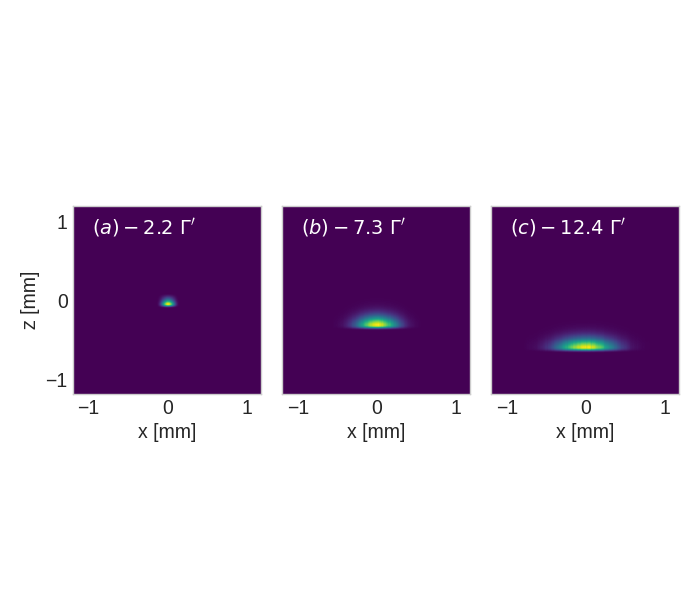
\includegraphics[width=0.9\textwidth]{USPSC-img/sr_loftus_cloud_profile.png}
    \vspace{5px}
    \legend{Simulated strontium cloud profile for three laser detunings: $ \delta = -5.0\Gamma' $ (a), $ \delta = -8.6\Gamma' $ (b), and $ \delta = -11.1\Gamma' $ (c), where $ \Gamma' = \Gamma \sqrt{1 + s_0} $ is the power-broadened linewidth. \\ Source: author}
    \label{fig:sr-loftus-atomic-cloud-profile}
\end{figure}

\begin{figure}[!ht]
    \centering
    \caption{Centre of mass of the ${}^{88}Sr$ nMOT as a function of the lasers detuning}
    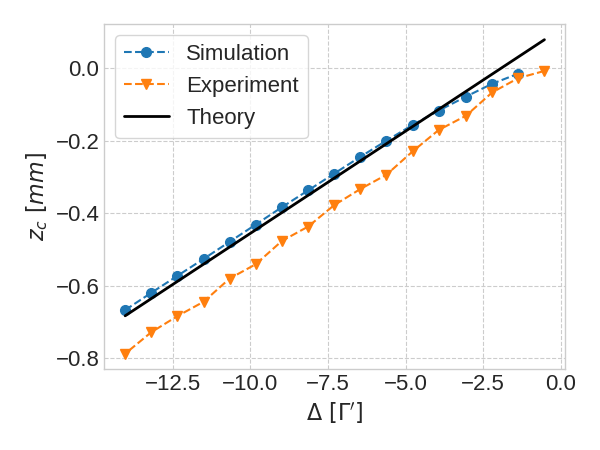
\includegraphics[width=0.6\textwidth]{USPSC-img/sr_centre_of_mass.png}
    \vspace{5px}
    \legend{centre of mass.\\ Source: author}
    \label{fig:sr-centre-of-mass}
\end{figure}

\begin{figure}[!ht]
    \centering
    \caption{Cloud size of the ${}^{88}Sr$ nMOT}
    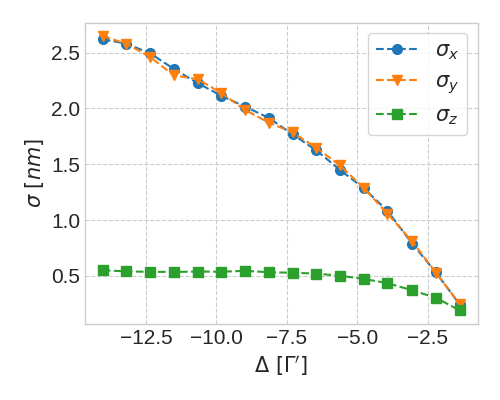
\includegraphics[width=0.8\textwidth]{USPSC-img/sr_loftus_cloud_size.png}
    \vspace{5px}
    \legend{cloud size.\\ Source: author}
    \label{fig:sr-loftus-cloud-size}
\end{figure}


%-----------------------------------
\subsection{Temperature}
\label{temperature}
%-----------------------------------

Experimental data from the \textit{strontium-ifsc}.

\begin{figure}[!ht]
    \centering
    \caption{Temperature of the ${}^{88}Sr$ nMOT as a function of the lasers detuning}
    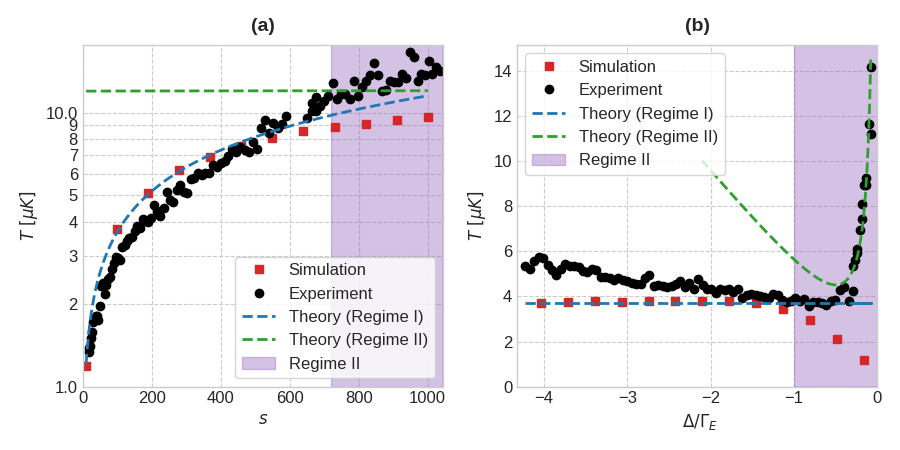
\includegraphics[width=1.0\textwidth]{USPSC-img/sr_temperature.png}
    \vspace{5px}
    \legend{temperature.\\ Source: author}
    \label{fig:sr-temperature}
\end{figure}

%-----------------------------------
%


	% ---
	%  Conclusion
	% ---
	%
%--- 
%-----------------------------------
\chapter{CONCLUSION}
\label{ch:conclusion}
%-----------------------------------
%--- 
%

In this Master's degree work, we proposed and implemented a Monte Carlo simulation to estimate experimental quantities of narrow-line magneto-optical traps. We essentially estimate the probability distributions of the atoms' position and velocity in the presence of laser light and a quadrupole magnetic field. Then, with these distributions, we estimate the atomic cloud profile and the temperature. Our proposal is to sample the atoms' states by considering their movement as a Markovian process.

We were able to simulate three nMOT arrangements reproduced by different laboratories and obtain estimated quantities that are more accurate than the theoretical ones. It is possible to use our simulation to optimize parameters of nMOTs without the necessity of experimental data. It is also a tool to analyse the feasibility of unusual nMOT arrangements such as nMOTs with fewer laser beams.

We analysed the limits of our model regarding the three nMOT regimes and verified that it works exclusively in the power-broadened regime. Therefore, to obtain accurate quantities, it is necessary to guarantee a set of parameters that keep the nMOT in this regime. We validated our model for nMOTs with small and slightly large narrownesses. It is possible to estimate quantities for both cases, but the larger the narrowness, the more difficult it is to reach the power-broadened regime. Hence, nMOTs with small narrownesses have a larger range in which we are able to predict experimental quantities. The nMOT setup with a slightly large narrowness must be designed to decrease the trapping effect in the gravity direction so that the atoms are able to fall under gravity. This is a typical effect of power-broadened nMOTs.

We confirmed that our simulation is capable of estimating quantities for complicated transitions by assuming the spin-polarized atoms. In our model, we are assuming that the transition is a four-level system. The dysprosium nMOT presented in Section \ref{sec:dysprosium} is based on an electronic transition with 36 states. Nevertheless, we were able to estimate quantities by assuming spin-polarized atoms based on previous works in which this phenomenon was observed experimentally.


%The magneto-optical traps are the workhorse of laser cooling. They were essential for at least two Nobel Prize laureates works since they allowed a myriad of remarkable achievements such as the Bose-Einstein condensation, accurate atomic clocks, quantum computers, and quantum sensors. Although MOTs work well experimentally, the theory of MOTs does not provide accurate predictions for some experimental quantities. The case of narrow-line MOTs is even more complicated due to the gravity effect.

%The first part of this work was focused on to understand the interaction between atoms and light, which is essential to study MOTs properly. from two approaches. The first one is the rate equations model proposed by Albert Einstein. We explored such approach to get start to basic concepts. The second approach is the optical Bloch equations, which contemplates coherent effects and fundamental understanding of the line broadening mechanisms. We then deduced and analysed the optical forces, which is a key concept to understand the theory of the magneto-optical trap. We introduced the MOT theory by an simply one-dimension model. Afterwards, we presented the three-dimensional case as well as the narrow-line magneto-optical trap.



	% ----------------------------------------------------------
	% Post-Textual Elements
	% ----------------------------------------------------------
	\postextual
	% ----------------------------------------------------------

	% -----------------------------------------------------------
	% Referências bibliográficas
	% ----------------------------------------------------------
	\bibliography{references}


	% ----------------------------------------------------------
	% Glossary
	% ----------------------------------------------------------
	%\glossary

	% ----------------------------------------------------------
	% Apêndices
	% ----------------------------------------------------------
	%
% Beggining of appendix
%-----------------------------------
\begin{apendicesenv}

% Zeeman splitting
%-----------------------------------
%%
%-----------------------------------
\chapter{Anomalous Zeeman effect}
\label{ap:anomalous-Zeeman-effect}
%-----------------------------------
%

The interaction between an external magnetic field and an atom splits the atomic energy levels\footnote{The atomic energy levels are negative energies associated with the bound between the electrons and the atomic nucleus.}. Let us consider, without loss of generality, a z-directed magnetic field $ \mathbf{B} = B \mathbf{e}_z $ and an atom whose magnetic dipole moment is $ \vec{\mu} $. We shall neglect the hyperfine structure so that $ \vec{\mu} = \vec{\mu}_{L} + \vec{\mu}_{S} $, being $ \vec{\mu}_{L} $ the orbital magnetic moment and $ \vec{\mu}_{L} $ the spin moment given by
\begin{align}
	\vec{\mu}_{L} &= -\frac{\mu_B g_L}{\hbar} \mathbf{L} & &\textrm{and} & \vec{\mu}_{S} &= -\frac{\mu_B g_S}{\hbar} \mathbf{S},
\end{align}
where $ \mu_B $ is the Bohr magneton, $ g_L = 1 $ and $ g_S = 2.002319314... \simeq = 2 $ are \textit{g-factors}, $ \mathbf{L} $ is the orbital angular momentum, and $ \mathbf{S} $ is the spin angular momentum. The interaction between the field $ \mathbf{B} $ and the atom is essentially dipolar such that it is described by the following Hamiltonian 
\begin{equation}
	\hat{V} = - \vec{\mu} \cdot \mathbf{B} = \frac{\mu_B}{\hbar}(\mathbf{L} + 2\mathbf{S}) \cdot \mathbf{B} = \frac{\mu_B B}{\hbar}(\hat{L}_z + 2 \hat{S}_z).
	\label{eq:dipolar-magnetic-interaction}
\end{equation}
The interaction energy $ \mu_B B $ is comparable with the atomic energy levels for astronomical magnetic fields of magnitude around $ 10^{5}\ T $. In most situations, we can safely assume this interaction as a \textit{perturbation}. Let us also assume the interaction energy much lower than spin-orbit coupling ($ < 1\ T $) so that the total angular momentum $ \mathbf{J}^2 = (\mathbf{S} + \mathbf{L})^2 $ and its z-projection $ \hat{J}_z = \hat{S}_z + \hat{L}_z $ are compatible observables\footnote{The spin-orbit coupling is described by a Hamiltonian $ \hat{H}_{so} \propto \mathbf{S} \cdot \mathbf{L} $. Since $ \hat{J}^2 = (\mathbf{S} + \mathbf{L}) = \hat{S}^2 + \hat{L}^2 + 2(\mathbf{S} \cdot \mathbf{L}) $, we have $ [\hat{H}_{so}, \hat{J}^2] = [\hat{H}_{so}, \hat{J}_z] = 0 $. Therefore, $ \hat{J}^2 $ and $ \hat{J}_z $ are compatibles with $ \hat{H}_{so} $.} with the unperturbed atomic Hamiltonian even under an external magnetic field. In this case, $ \mathbf{B} $ is said to be a weak field. From the \textbf{perturbation theory}, the \textit{first order} energy correction is given by
\begin{align}
	\Delta E &= \frac{\mu_B B}{\hbar}\braket{n, l, s, j, m_j|\hat{L}_z + 2\hat{S}_z|n, l, s, j, m_j} \\
	&= \frac{\mu_B B}{\hbar} (\braket{n, l, s, j, m_j|\hat{J}_z|n, l, s, j, m_j} + \braket{n, l, s, j, m_j|\hat{S}_z|n, l, s, j, m_j}),
\end{align}
where $ n $ is the \textit{principal quantum number} and $ l $, $ s $, $ j $, and $ m_j $ are quantum numbers associated with the angular momenta: \textit{orbital} $ \hat{L}^2 $, \textit{spin} $ \hat{S}^2 $, \textit{total} $ \hat{J}^2 $, and z-projection $ \hat{J}_z $. By the \textbf{Wigner-Eckart theorem}, we have
\begin{equation}
	\braket{n, l, s, j, m_j|\hat{L}_z + 2\hat{S}_z|n, l, s, j, m_j} = g
\end{equation}
%-----------------------------------

\end{apendicesenv}
%-----------------------------------

	% ----------------------------------------------------------
	% Anexos
	% ----------------------------------------------------------
	%%% USPSC-Anexos.tex
% ---
% Inicia os anexos
% ---
\begin{anexosenv}

% Imprime uma página indicando o início dos anexos
\partanexos

% ---
\chapter{Exemplo de anexo}
% ---
Elemento opcional, que consiste em um texto ou documento não elaborado pelo autor, que serve de fundamentação, comprovação e ilustração, conforme a ABNT NBR 14724. \cite{nbr14724}.

O \textbf{ANEXO B} exemplifica como incluir um anexo em pdf.

\chapter{Acentuação (modo texto - \LaTeX)}
\begin{figure}[H]
	\begin{center}
	\caption{\label{fig_anexob}Acentuação (modo texto - \LaTeX)}
	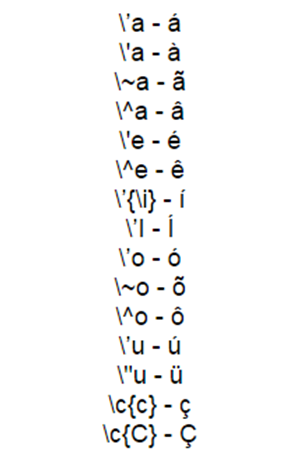
\includegraphics[scale=1.0]{USPSC-img/USPSC-AcentuacaoLaTeX.png} \\
	Fonte: \citeonline{comandos}
	\end{center}	
\end{figure}

\end{anexosenv}


	%---------------------------------------------------------------------
	% INDICE REMISSIVO
	%--------------------------------------------------------------------
	%%% USPSC-IndicexRemissivosTutorial.tex
% ---
% Inicia os Índices Remissivos
% ---
%---------------------------------------------------------------------
% INDICE REMISSIVO
%--------------------------------------------------------------------
\phantompart
\printindex
%---------------------------------------------------------------------


	%---------------------------------------------------------------------
\end{document}
% ---
